\documentclass[UTF8]{ctexart}
\usepackage{mathtools,booktabs}
\usepackage{graphicx}
%添加路径,图片的搜索路径
\graphicspath{{figures/}}
\usepackage{listings} 
\usepackage{xcolor}
\lstset{
	language=c,  %代码语言使用的是matlab
	frame=shadowbox, %把代码用带有阴影的框圈起来
	rulesepcolor=\color{red!20!green!20!blue!20},%代码块边框为淡青色
	keywordstyle=\color{blue!90}\bfseries, %代码关键字的颜色为蓝色,粗体
	commentstyle=\color{red!10!green!70}\textit,    % 设置代码注释的颜色
	showstringspaces=false,%不显示代码字符串中间的空格标记
	numbers=left, % 显示行号
	numberstyle=\tiny,    % 行号字体
	stringstyle=\ttfamily, % 代码字符串的特殊格式
	breaklines=true, %对过长的代码自动换行
	extendedchars=false,  %解决代码跨页时,章节标题,页眉等汉字不显示的问题
	%   escapebegin=\begin{CJK*},escapeend=\end{CJK*},      % 代码中出现中文必须加上,否则报错
	texcl=true}


\begin{document}
	
	\title{八股文背诵合集}
	\author{The Sea and Sheng}
	\maketitle
	
	\tableofcontents
	\newpage
	
	\section{Spring}
	%\subsection{二级标题}
	\subsubsection{Spring 框架能带来哪些好处}

	\begin{enumerate}
		\item Dependency Injection(DI) 依赖注入 是的构造器和JavaBean properties文件中的依赖关系一目了然.
		\item IoC容器更加趋向于轻量级.
	\end{enumerate}
\subsubsection{如何实现AOP, 项目那些地方用到了AOP}
利用JDK动态代理或Cglib动态代理, 利用动态代理技术, 可以针对某个类生成代理对象, 当调用代理对象的某个方法时, 可以任意控制该方法的执行, 比如可以先打印执行时间, 再执行该方法, 并且该方法执行完成后, 再次打印执行时间. \par
权限管理是使用AOP技术实现的. 凡是需要对某些方法做统一处理的都可以用AOP来实现, 利用AOP可以做到业务的无侵入 \par
\subsubsection{Spring的事物机制}
1. Spring事物机制底层是基于数据库事物和AOP机制的 \par
2. 首先对于使用了@Transactional注解的bean, spring会创建一个代理对象作为Bean \par
3. 当调用代理对象的方法时, 弧线判断方法上是否加了@Transactional注解 \par
4. 如果加了, 那么则利用事物管理器创建一个数据库连接 \par
5. 并且修改数据库连接的autocommit属性为false, 禁止此连接的自动提交, 这是实现Spring事物非常重要的一步. \par
6. 然后执行当前方法, 方法中会执行sql \par
7. 执行完当前方法后, 如果没有出现异常就直接提交事物 \par
8. 如果出现了异常, 并且这个异常是需要回滚的就会回滚事物, 否则仍然提交事物 \par
9. Spring事物的隔离级别对应的就是数据库的隔离级别 \par
10. Spring事物的传播机制是Spring事物自己实现的, 也是Spring事物中最复杂的. \par
11. Spring事物的传播机制是基于数据库连接来做的, 一个数据库连接一个事物, 如果传播机制配置为需要新开一个事物, 那么实际上就是先建立一个数据库连接, 在此新数据库连接上执行sql.
\subsubsection{Spring什么时候@Transactional失效}
如果某个纺纱是private的, 那么@Transactional也会失效, 因为底层calib是基于父子类来实现的, 子类是不能重载父类的private方法的, 所以无法很好的利用代理, 也会导致@Transactional失效 \par
\subsubsection{介绍一下Spring, 读过源码介绍一下大致流程}
1. Spring是一个快速开发框架, Spring帮助程序员来管理对象 \par
2. Spring的源码实现的是非常优秀的, 设计模式的应用, 并发安全的实现, 面向接口的设计等 \par
3. 在创建Spring容器, 也就是启动Spring时: \par
a. 首先会进行扫描, 骚婊得到所有的BeanDefinition对象, 并存在一个Map中 \par
b. 然后筛选出非懒加载的单例BeanDefinition进行创建Bean, 对于多例Bean不需要再启动过程中去进行创建, 对于多例Bean会在每次获取Bean时利用beanDefinition去创建 \par
c. 利用beanDefinition创建Bean就是Bean的创建生命周期, 这期间包括了合并BeanDefinition, 推断构造方法, 实例化, 属性填充, 初始化前, 初始化, 初始化后等步骤, 其中AOP就是发生在初始化后这一步骤中\par
4. 单例Bean创建完了之后, Spring会发布一个容器启动事件. \par
5. Spring启动结束 \par

\subsubsection{Autowired}
使用byType和byName去寻找需要进行注入的对象
	\subsubsection{什么是控制反转(IOC)}
	\begin{enumerate}
		\item 
		控制反转简单来说, 以前程序开发的时候, 是由程序员通过new来生成对象. 在使用控制反转的情况下, 对象的实例化由Spring框架中的IoC容器来控制对象的创建; 
		\item 由容器来管理这些对象的生命周期.
		\item Spring中的org.springframework.beans包和org.springframework.conext包构成了Spring框架Ioc的基础. 主要使用文件 applicationContext.xml 来进行配置.
	\end{enumerate}

	\subsubsection{什么是依赖注入?}
	\begin{enumerate}
		\item Spring 通过反射来实现依赖注入
		\item 当我们需要某个功能比如Connection, 至于Connection怎么构造, 何时构造我们不需要知道. 在系统运行时, Spring会在适当的时候制造一个Connection, 我们需要一个Connection, 这个Connection是由Sping注入到A中. 
	\end{enumerate}
\subsubsection{Spring 对对象进行创建流程}
class对象反射 ---> 实例化 ---> 生成对象 ---> 属性填充(依赖注入)  ---> 初始化(afterPropertiesSet) ---> AOP ---> 代理对象(cglib) ---> bean
\subsubsection{什么是AOP}
允许横切业务, 由切面构成, 切面又切入点和通知构成,@Aspect注解的类就是切面. \par
(1) 目标对象(Target) \par
要被增强的对象. \par
(2) 连接点, 哪个目标方法, 相对点, 目标方法的前还是后.
\subsubsection{bean的生命周期}
什么是bean? \par
从上面可知,我们可以给Bean下一个定义:Bean就是由IOC实例化、组装、管理的一个对象。
\begin{figure}
	\centering
	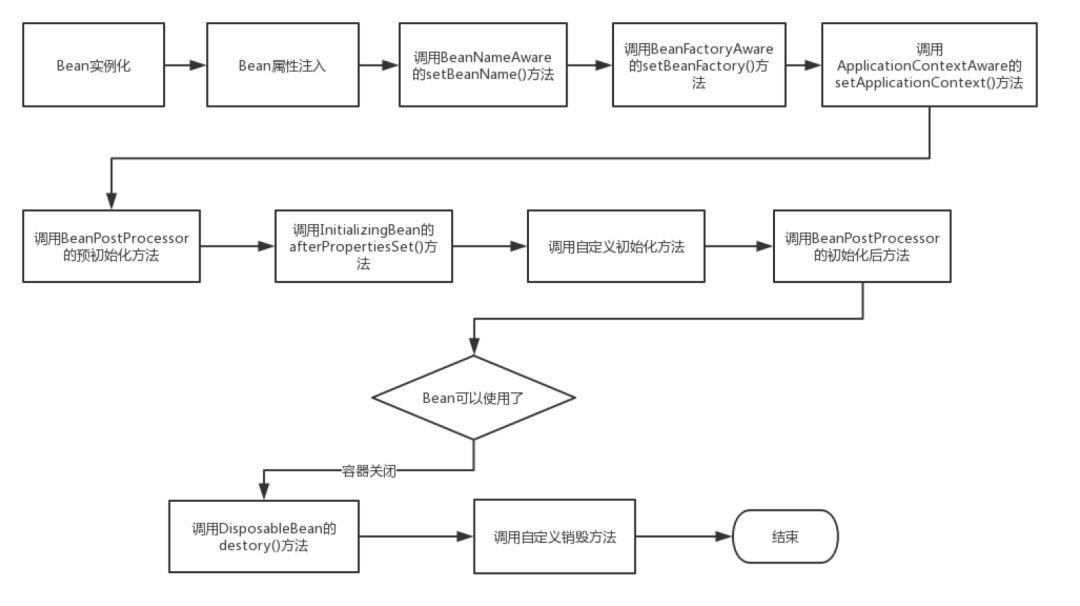
\includegraphics[width=0.7\linewidth]{figures/bean_live.jpg}
	\caption{}
	\label{fig:bean_live}
	
\end{figure}
如上图所示,Bean 的生命周期还是比较复杂的,下面来对上图每一个步骤做文字描述: \par
(1) Spring启动,查找并加载需要被Spring管理的bean,进行Bean的实例化 \par
(2) Bean实例化后对将Bean的引入和值注入到Bean的属性中 \par
(3) 如果Bean实现了BeanNameAware接口的话,Spring将Bean的Id传递给setBeanName()方法 \par
(4) 如果Bean实现了BeanFactoryAware接口的话,Spring将调用setBeanFactory()方法,将BeanFactory容器实例传入 \par
(5) 如果Bean实现了ApplicationContextAware接口的话,Spring将调用Bean的setApplicationContext()方法,将bean所在应用上下文引用传入进来。 \par
(6) 如果Bean实现了BeanPostProcessor接口,Spring就将调用他们的postProcessBeforeInitialization()方法。\par
(7) 如果Bean实现了InitializingBean接口,Spring将调用他们的afterPropertiesSet()方法。类似的,如果bean使用init-method声明了初始化方法,该方法也会被调用 \par

(8) 如果Bean 实现了BeanPostProcessor接口,Spring就将调用他们的postProcessAfterInitialization()方法。\par
(9) 此时,Bean已经准备就绪,可以被应用程序使用了。他们将一直驻留在应用上下文中,直到应用上下文被销毁。\par
(10) 如果bean实现了DisposableBean接口,Spring将调用它的destory()接口方法,同样,如果bean使用了destory-method 声明销毁方法,该方法也会被调用。\par
\subsubsection{简单阐述SpringMVC的流程}
	SpringMVC是一个基于Java的实现了MVC设计模式的请求驱动类型的轻量级Web框架, 通过把Model, View, Controller分离, 将web层进行职责解耦, 把复杂的web应用分成逻辑清晰的几部分, 简化开发.
\par
(1) 用户发送请求到前端控制器DispatcherServlet;
\par
(2) DispatcherServlet 收到请求后, 调用HandlerMapping处理器映射器, 请求获取Handle
\par
(3) 处理器映射器更具请求url找到具体的处理器, 生成处理器对象以及处理器拦截器(如果有则生成)一并返回给DispatcherServlet;
\par
(4) DispatcherServlet 调用HandlerAdapter处理器适配器;
\par
(5) HandlerAdapter 经过适配调用具体处理器(Handler, 也叫后端控制器);
\par
(6) Handler 执行完成返回ModelAndView;
\par
(7) HandlerAdapter将Handler执行结果ModelAndView返回给DispatcherServlet;
\par
(8) DispatcherServlet将ModelAndView传给ViewResolver视图解析器进行解析;
\par
(9) ViewResolver解析后返回具体View
\par
(10) DispatcherServlet对View进行渲染视图(即将模型数据填充到视图中)
\par
(11) DispatcherServlet响应用户.
\par
简单来说, 我们需要开发的就是 == 开发处理器(Handler,即我们的Controller, 对于视图jsp我们前后端分离之后也不用写了.
\begin{figure}
	\centering
	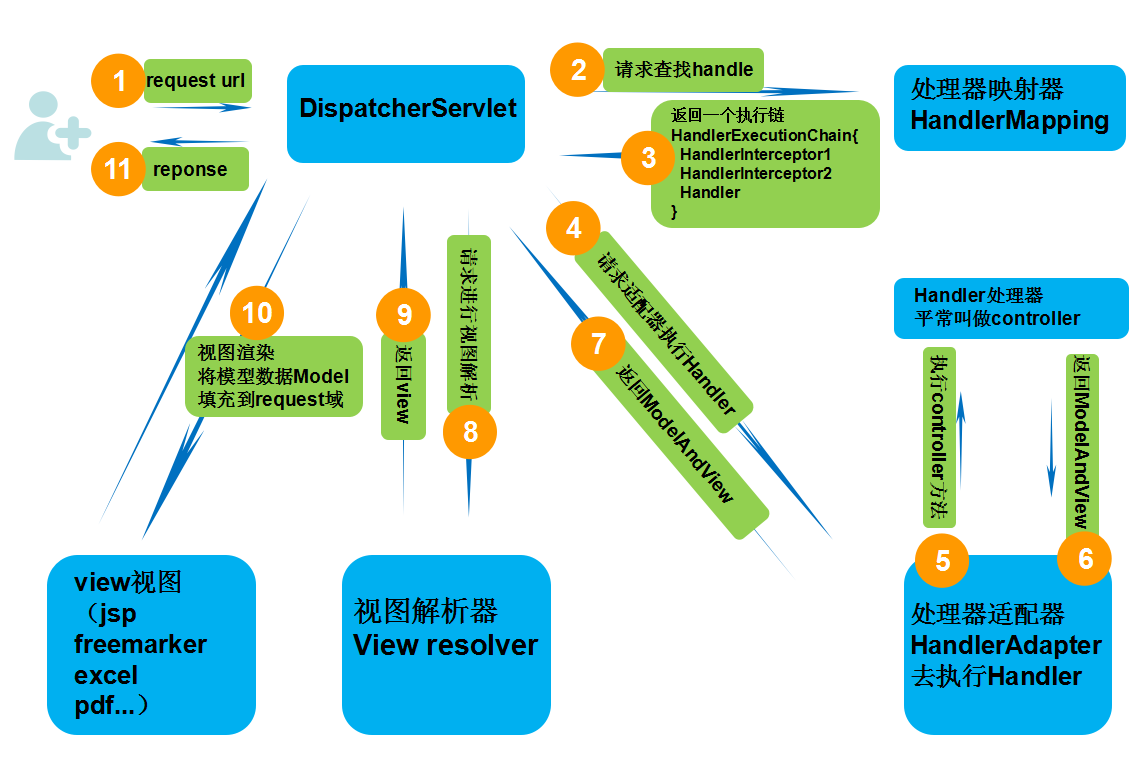
\includegraphics[width=0.7\linewidth]{figures/SpringModelAndView.png}
	\caption{}
	\label{fig:SpringModelAndView}
\end{figure}
	\subsubsection{第三个三级标题}
	
	
\section{java基础}
%\subsection{二级标题}
\subsubsection{hashmap死锁产生情况}
1.7 版本的死锁是在 rehash方法中的transfer方法产生的, 因为在扩容的过程中, 主要关于两个指正, e指正指向当前节点, next是e的下一个指针, 因为采用头插法会前后顺序调换, 导致产生换的现象. \par
\subsubsection{谈谈对ConcurrentHashMap的扩容机制}
1.7版本: \par
1. 1.7版本的ConcurrentHashmap是基于Segment分段实现的\par
*. Segment 依赖 ReentrantLock实现 \par
2. 每个Segment(数组)相对于一个小型的Hashmap \par
3. 每个Segment内部会进行扩容, 和hashMap的扩容逻辑类似 \par
4. 先生成新的数组, 然后转移元素到新数组中 \par
5. 扩容的判断也是每个Segment内部单独判断的, 判断是否超过阈值 \par
1.8版本 \par
1. ConcurrentHashMap 不再基于Segment实现 \par
2. 当某个线程运行put时候, 如果发现ConcurrentHashMap 正在进行扩容, 那么该线程一起进行扩容 \par
3. 如果某个线程,put时, 发现并没有正在进行扩容, 则将keyvalue添加到ConcurrentHashMap中, 然后判断是否超过阈值, 超过则进行扩容 \par
4. concurrentHashMap是支持多个线程同时扩容的 \par
5. 扩容之前也先生成一个新的数组 \par
6. 在转移元素时, 先将原数组分组, 将每组分给不同的额线程来进行元素转移, 每个线程负责一组或多组的元素转移工作. \par
\subsubsection{造成死锁的原因}
1. 若干线程形成头尾相接的循环等待资源关系 \par
\textbf{解决方案:} \par
1. 注意加锁的顺序, 保证每个线程按照同样的顺序进行加锁 \par
2. 要注意加锁的时间, 可以针对锁设置一个超时时间 \par
3. 要注意死锁检查, 这是一种预防机制, 确保在第一时间发现死锁并进行 \par
4. 使用jstack 来查看dump 文件 \url{https://blog.csdn.net/u010647035/article/details/79769177}, 来查看锁的依赖关系 \par
5. 避免一个线程使用多个锁 \par
6. 尝试使用定时锁, 使用lock.tryLock(timeout)来代替使用内部锁 \par
7. 对于数据库锁, 加锁和解锁必须在用一个数据连接里, 否则会出现锁失效的情况 \par
\subsubsection{深拷贝和浅拷贝}
1. 一个对象中存在两种数据类型的属性, 一种是基本数据类型, 一种是实例对象的引用 \par
A. 浅拷贝是指, 只会拷贝基本数据类型的值, 以及实例对象的引用地址, 并不会复制一份引用地址所指向的对象, 也就是浅拷贝出来的对象, 内部的属性指向的是同一个对象 \par
B. 深拷贝是指, 既会拷贝基本数据类型的值, 也会针对实例对象的引用地址所指向的对象进行赋值, 深拷贝出来的对象, 内部的类执行指向的不是同一个对象 \par
\subsubsection{如果你提交任务时, 线程池队列已满, 这时会发生什么}
1. 如果使用的是无界队列, 那么可以继续提交任务 \par
2. 如果使用有界队列, 提交任务时, 如果队列满了, 如果线程数小于最大线程数, 那么增加线程, 如果线程数已经达到了最大值, 则使用拒绝策略进行拒绝 \par
\subsubsection{遇到过哪些设计模式}
1. 代理模式, Spring中的AOP使用了代理模式 \par
2. 工厂模式, Spring的BeanFactory就是一种工厂模式的实现 \par
\subsubsection{Spring中Bean是线程安全的吗?}
Spring本身并没有针对bean做线程安全处理, 所以 \par
1. 如果Bean是无状态的, 那么Bean则是线程安全的 \par
2. 如果Bean是有状态的, 那么Bean则不是线程安全的

\subsubsection{说说你了解的分布式锁实现}
分布式锁所要解决的问题的本质是: 能够对分布在多台季启忠的线程对共享资源的互斥访问. 在这个原理上可以有很多的实现方式 \par
1. 基于Redis, Redis中的数据也是在内容, 基于原子操作比如setnx \par
2. jmeter 压测工具 \par
3. 使用setnx+过期时间, 使用 try + finally(来释放锁) 同时生成UUID(value), 自己使用的锁,自己释放, 防止自己的锁, 被别的进程释放 \par
4. 补充, 自动延时() \par
5. redisson() \par
\begin{figure}
	\centering
	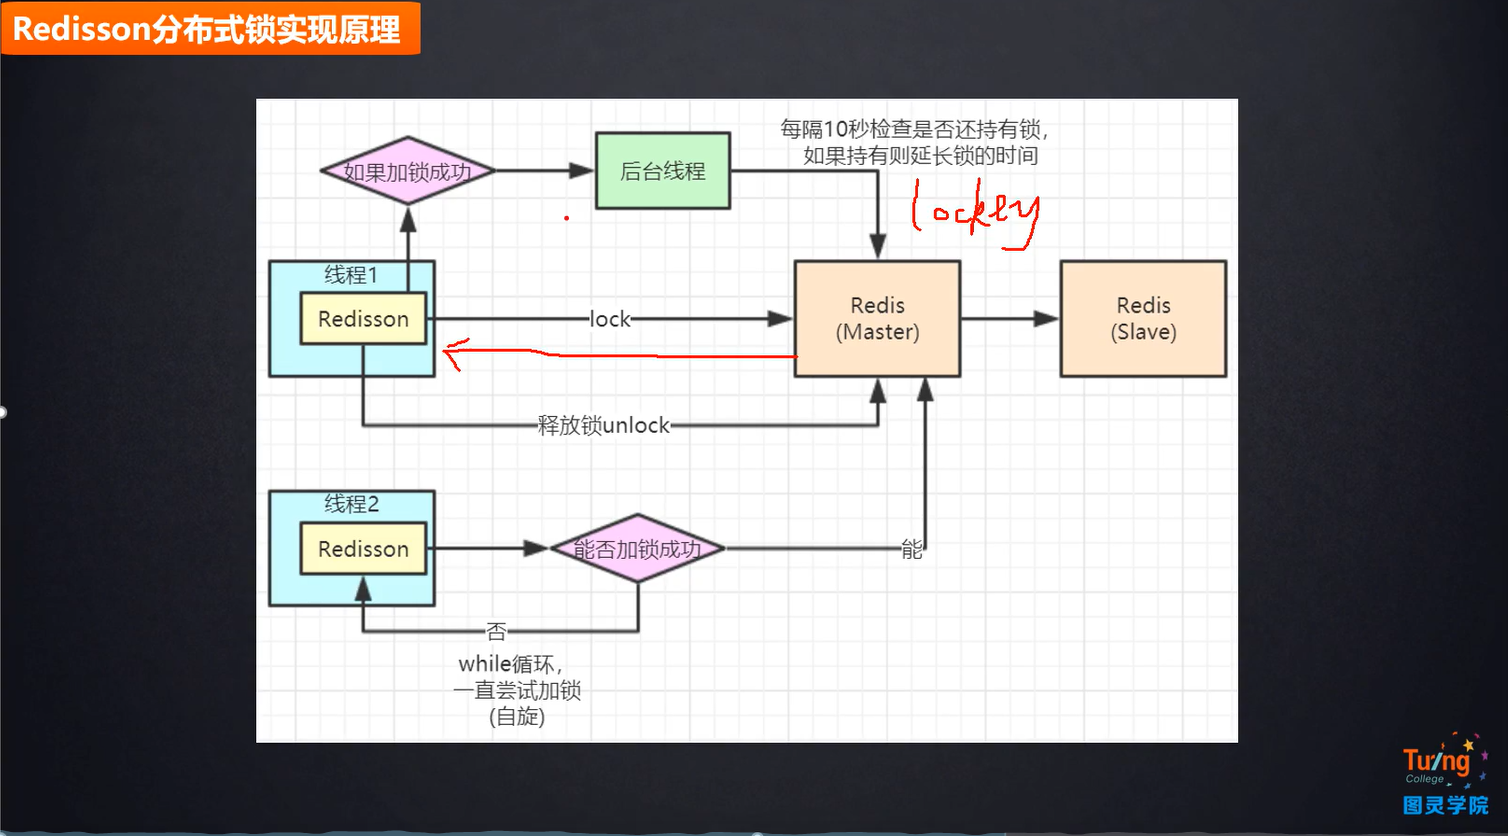
\includegraphics[width=0.7\linewidth]{figures/redission.png}
	\caption{}
	\label{fig:redission}
\end{figure}
\subsubsection{如何查看线程死锁}
0. 使用ps H -eo pid,tid,\%cpu|grep 2783 可以查看java进程中的线程
1. 使用jstack命令来查看 \par
2. 对于mysql 使用select * from INFOMATION\_SCHEMA.INNODB\_LOCKS 查看正在锁的事物 \par
3. 查看等待锁的事物 SELECT * FROM INFORMATION\_SCHEMA.INNODB\_LOCK\_WAITS \par
\subsubsection{线程之间如何进行通讯的}
1. 使用共享内存或基于网络来进行通信 \par
2. 如果是通过共享内存来进行通信
\subsubsection{快速失败(fail-fast) 和 安全失败(fail-safe) 的区别是什么?}
\begin{enumerate}
	\item java.util包下面的所有的集合类都是快速失败的, 而java.util.concurrent包下面的所有类都是安全失败的. 快速失败的迭代器会抛出ConcurrentModificationException异常, 而安全失败的迭代去永远不会抛出这样的异常.

\end{enumerate}
\subsubsection{异常}
(1) Throwable(可抛出) 超类, 有两个子类Error 和 exception 错误和异常
\subsubsection{synchronized的底层实现细节}
1. synchronized作用 \par
原子性: synchronized保证语句内操作是原子的 \par
可见性: synchronized保证可见性(通过在执行unlock之前, 必须先报此变量同步回主内存实现) \par
有序性: synchronized保证有序性(通过"一个变量在同一时刻只允许一条线程对其进行lock操作") \par
可见性补充: 	其实真正解决这个问题的是JMM关于Synchronized的两条规定: 
\par
1、线程解锁前,必须把共享变量的最新值刷新到主内存中; \par
2、线程加锁时,讲清空工作内存中共享变量的值,从而使用共享变量是需要从主内存中重新读取最新的值(加锁与解锁需要统一把锁) \par
\subsubsection{线程池参数}
ThreadPoolExecutor的创建参数: \par
(1) corePoolSize, 核心运行的线程个数, 若线程池已创建的线程数小于corePoolSize, 即使此时存在空闲线程, 也会通过创建一个新线程来执行该任务. \par
(2) maximumPoolSize: 最大线程个数, 当大于这个值就会将准备新加入的异步任务有一个丢弃处理机制来处理, 大于corePoolSize且小于maxmumPoolSize存入等待队列,\par
(3) workQueue: 任务等待队列, 当达到corePoolSize的时候就向该等待队列放入线程信息.\par
(4) keepAliveTime: 默认0, 当线程没有任务处理后空闲线程保持多长时间, 不推荐使用, 一般会中止超过corePoolSize数量的线程资源, 空闲线程时间超过keepAliveTime, 线程将会被回收 \par
(5) threadFacory: 构造Thread方法, 使用默认的default实现. \par
(6) defaultHandler: 当maximumPoolSize达到后丢弃处理的方法实现, java默认是丢出异常. \par
\subsubsection{sychronized和ReentrantLock的区别}
1. sychronized是一个关键字, ReentrantLock是一个类 \par
2. synchronized会自动的加锁和释放锁, ReentrantLock是一个类 \par
3. sychronized的底层是jvm层面的锁, ReentrantLock是API层面的锁 \par
4. sychronized是非公平锁, ReentrantLock可以选择公平锁或非公平锁 \par
5. sychronized锁的是对象, 锁信息保存在对象头中, ReentrantLock锁的是线程 \par
6. sychronized底层有一个锁升级的过程 \par
\subsubsection{线程池中使用的BlockQueue} 
(1) 直接提交队列: 简单来说使用SynchronousQueue队列,提交的任务不会被保存,总是会马上提交执行。如果用于执行任务的线程数量小于maximumPoolSize,则尝试创建新的进程,如果达到maximumPoolSize设置的最大值,则根据你设置的handler执行拒绝策略。因此这种方式你提交的任务不会被缓存起来,而是会被马上执行,在这种情况下,你需要对你程序的并发量有个准确的评估,才能设置合适的maximumPoolSize数量,否则很容易就会执行拒绝策略;\par
(2) 有界的任务队列可以使用ArrayBlockingQueue实现,若有新的任务需要执行时,线程池会创建新的线程,直到创建的线程数量达到corePoolSize时,则会将新的任务加入到等待队列中。若等待队列已满,即超过ArrayBlockingQueue初始化的容量,则继续创建线程,直到线程数量达到maximumPoolSize设置的最大线程数量,若大于maximumPoolSize,则执行拒绝策略。在这种情况下,线程数量的上限与有界任务队列的状态有直接关系,如果有界队列初始容量较大或者没有达到超负荷的状态,线程数将一直维持在corePoolSize以下,反之当任务队列已满时,则会以maximumPoolSize为最大线程数上限。\par
(3) 使用无界任务队列,LinkedBlockingQueue 实现线程池的任务队列可以无限制的添加新的任务,而线程池创建的最大线程数量就是你corePoolSize设置的数量,也就是说在这种情况下maximumPoolSize这个参数是无效的,哪怕你的任务队列中缓存了很多未执行的任务,当线程池的线程数达到corePoolSize后,就不会再增加了;若后续有新的任务加入,则直接进入队列等待,当使用这种任务队列模式时,一定要注意你任务提交与处理之间的协调与控制,不然会出现队列中的任务由于无法及时处理导致一直增长,直到最后资源耗尽的问题。 \par
(4) 优先任务队列:优先任务队列通过PriorityBlockingQueue实现,
\subsubsection{Executors 工厂类实现线程池}
通过创建不同的ThreadPoolExecutor参数.\par
(1) FixedThreadPool 定长, corePoolSize == maxmumPoolSize   \par
(2) SingleThreadExecutor 单一线程 无界队列 \par
以上两种可能会堆积大量的请求, 从而引起OOM异常 \par
(3) CachedThreadPool 采用maxmumPoolSize为无限大, 容易创建大量线程, 从而耗尽系统资源. \par

\subsubsection{线程池的拒绝策略}
(1) abortPolicy 默认: 直接抛出异常 \par
(2) CallerRunsPolicy:  直接调用主线程来执行任务. \par
(3) DiscardPolicy: 不能执行的任务被删除, 和abortPolicy一样, 但是不抛出异常. \par
(4) DiscardOldestPolicy: 位于工作队列头部的任务将被删除, 然后重新执行程序. \par
\subsubsection{8种基本数据类型}
\begin{table}[!htbp]
	\centering
	\caption{实现}
	\begin{tabular}{|l|r|}
		
		\hline
		类型&大小(注释/包装类)\\
		\hline
		byte&8(Byte)\\
		\hline
		short&16(Short)\\
		\hline
		int&32(Integer)\\
		\hline
		long&64(Long)\\
		\hline
		float&32(Float)\\
		\hline
		double&64(Double)\\
		\hline
		char&16(Character)\\
		\hline
		boolean&8(Boolean)\\
		\hline
	\end{tabular}
\end{table}
\subsubsection{Comparable \& Comparator 区别}
Comparable 是接口 能力赋予
\begin{lstlisting}
public interface Comparable<T> {
	public int compareTo(T o);
}
\end{lstlisting}
Comparator 是外部比较器, 也是接口, 类似于 C++sort中自定义的cmp函数
\begin{lstlisting}
Collections.sort(list, new Comparator<Person2>() {
	public int compare(Person o1, Person o2) {
		return o1.getAge() - o2.getAge();
	}
})
\end{lstlisting}
\subsubsection{java采用值传递还是引用传递?}
采用值传递, 但是因为采用浅拷贝, 所以会修改传递的对象的相关属性.
\subsubsection{java深拷贝和浅拷贝}
实现了Coneable接口实现深拷贝.
\subsubsection{java"==" 和 equals 的区别}
1. "==" : 如果是基本数据类型, 则直接对值进行比较, 如果是引用数据类型, 则是对他们的地址进行比较;
\par
2. equals方法继承Object类, 在具体实现时可以覆盖父类中的实现. 看一下Object中equals的源码发现, 它的实现也是对\textbf{对象的地址}进行比较, 可以覆盖实现这个方法, 如果两个对象的类型一致, 并且内容一致, 则返回true.
\par
在实际开始中总结:
\par
(1) 类未复写equals, 则使用equals方法比较两个对象时, 相当于==比较, 及两个地址是否相等. 地址相等, 返回true, 地址不相等, 返回false.
\par
(2) 类复写equals方法, 走复写之后的判断方式. 通常, 我们会将equals复写成: 当两个对象内容相同时, 则equals返回true, 内容不同时, 返回false.
\par
对于set, hashMap, hashset等, 还要重写hashCode值, 比如set判断两个元素是否相等的时候, 会判断hashcode和equals都相等, 则认为相等, 不会添加新元素.
\subsubsection{String和StringBuilder, StringBuffer的区别}
String是不可变字符串对象(final的char数组), StringBuilder和StringBuffer(线程安全)是可变字符串对象.
\par
为什么String是final修饰的?
\par
1. 为了实现字符串池, 因为只有当字符串是不可变的, 字符串池才有可能实现.
\subsubsection{Java反射机制}
简单来说就是在, 运行状态中, 对于任意一个类, 都能够知道这个类的所有属性和方法; 对于任意一个对象, 都能够调用它的任意方法和属性; 并且能改变它的属性. 这种动态获取的信息以及动态调用对象的方法的功能称为Java语言的反射机制.
\par
优点: 代码灵活度提高
\par
缺点: 性能瓶颈, 性能较慢.
\subsubsection{简述面向对象三大特征, 继承, 封装, 多态}
1. 封装
\par
简单来说, 就是使用private方法将没有必要暴露的方法和属性进行隐藏.
\par
2. 继承
\par
继承是从已有的类中派生出行的类, 减少代码冗余. 
\par
3. 多态
\par
父类引用指向不同子类对象.
\subsubsection{多态}
一般使用instance of 来判断对象的子类关系. 增加向下转型的健壮度. \par
\subsubsection{内部类}
(1) 静态内部类访问外部变量必须是静态的. \par
(2) 
\subsubsection{红黑树}
一般考察红黑树: 只考察概念.
\begin{figure}
	\centering
	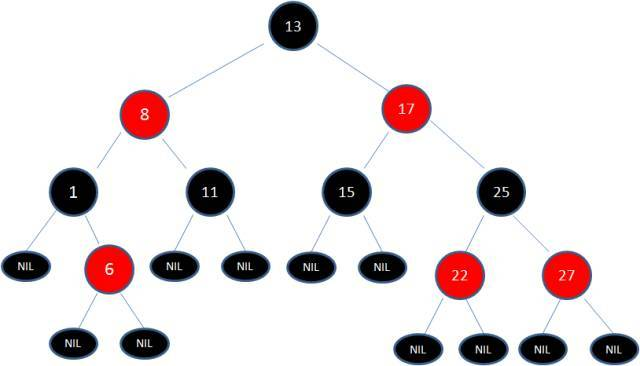
\includegraphics[width=0.7\linewidth]{figures/red_black.jpg}
	\caption{}
	\label{fig:jvm_copy}
\end{figure}
\begin{enumerate}
	\item 节点是红色或黑色
	\item 根节点是黑色
	\item 所有叶子都是黑色(叶子是NIL节点).
	\item 每个红色节点必须有两个黑色节点
	\item 从任一节点到其每个叶子的所有简单路径都包含相同数目的黑色节点.
	
\end{enumerate}

\subsubsection{hashmap的数据结构}
\begin{enumerate}
	\item jdk1.7 由 数组 + 链表  来构成
	\item jdk1.8 由 数组 + 链表 + 红黑树 来构成
	\item jdk1.8的时候, 当元素不超过64个的时候, 不会出现链表转红黑树, 当元素超过64个的时候, 会出现链表转红黑树.
	\item jdk1.8 当链表长度达到8个的时候, 链表会转为红黑树, 当红黑树元素长度退回到6个的时候会出现红黑树转为链表.
	\item jdk1.7 采用头插法, jdk1.8采用尾插法.
\end{enumerate}
\subsubsection{hashmap的put方法}
1. 根据Key通过哈希算法与与运算得到数组下标 \par
2. 如果数组下标位置元素为空, 则将key和value封装为Entry对象并放入该位置 \par
3. 如果数组下标元素不为空 \par
1.7, 则先判断是否需要扩容, 如果要扩容就进行扩容, 如果不用扩容就生成Entry对象, 并使用头茶法添加到当前位置的链表中 \par
1.8 先判断当前位置上Node的类型, 看是红黑树Node还是链表Node \par
a. 如果是红黑树Node, 则将key和value 封装为一个红黑树节点并添加到红黑树中 \par
b. 如果是链表节点, 使用尾插法插入到链表的最后位置去, 插入完后会判断当街链表的个数看是否需要转为红黑树(超过8个)元素. \par
c. 判断是否需要扩容(0.75*16默认值), 需要扩容就扩容, 不需要就结束PUT方法 \par
\subsubsection{介绍一下ThreadLocal} 
1. ThreadLocal 是java中所提供的的线程本地存储机制, 可以利用该机制将数据缓存在某个线程内部, 该线程可以在任意时刻, 任意方法中获取缓存的数据 \par
2. ThreadLocal 底层是通过ThreadLocalMap来实现的, 每个Thread对象中都存在一个ThreadLocalMap, Map的key为ThreadLoacl对象, Map的value为需要缓存的值 \par
3. 如果在线程池中使用ThreadLocal会造成内存泄露, 因为当ThreadLocal对象使用完后, 应该要报设置的key, value 也就是Entry对象进行回收, 但线程池中的线程不会回收, 而线程对象是通过强引用指向ThreadLocalMap, ThreadLocalMap也是通过强引用指向Entry对象, 线程不被回收, Entry对象也就不会被回收, 从而出现内存泄露, 解决方法是, 在使用了ThreadLocal对象之后, 手动调用ThreadLocal的remove方法, 手动清除Entry对象. \par
\subsubsection{heap和stack有什么区别}
\begin{enumerate}
	\item java的内存分为两类, 一类是堆内存, 一类是栈内存
	\item 栈内存是指程序进入一个方法时, 会为这个方法单独分配一块私属存储空间, 用于存储这个方法内部的局部变量. 当这个方法结束时, 分配给这个方法的栈会释放, 这个栈中的变量也随之释放.
	\item 使用new创建的对象存放在堆里, 不会随方法的结束二小时. 方法中的局部变量使用final修饰后, 放在堆中, 而不是栈中.
	
\end{enumerate}

\subsubsection{Array 和 ArrayList 的区别}
\begin{enumerate}
	\item Array 大小固定, ArrayList 大小是动态变化的.
\end{enumerate}
\subsubsection{Java各种锁: 悲观锁, 泪管所, 自旋锁, 偏向锁, 轻量/重量锁, 读写锁, 可重入锁}
悲观锁和乐观锁指的是并发情况下的两种不同策略, 是一种宏观的描述.
\par

\begin{enumerate}
	\item 悲观锁和乐观锁指的是并发情况下的两种不同策略, 是一种宏观的描述.
	
\end{enumerate}
\subsubsection{Collection 和 Collections 的区别}
\begin{enumerate}
	\item Collection 是集合类的上级接口, 继承他的接口主要是set和list
	\item Collections 类数针对集合类的一个帮助类. 它提供了一系列的静态方法对各种集合的搜索, 排序, 线程安全化等操作.
\end{enumerate}
\subsubsection{接口与抽象类区别}
\begin{enumerate}
	\item 类可以实现多个接口但只能继承一个抽象类
	\item 接口中变量被隐性制定为public static final, 方法被指定为 public abstract
	\item 接口里面所有的方法都是Public的, 抽象类允许Private, Protected方法
	\item JDK接口可以实现默认方法和静态方法, 前面加defalut, static关键字.
	\item 设计层面: 抽象类是对事物的抽象, 接口是对行为的抽象.
\end{enumerate}
\begin{lstlisting}
public interface InterfaceJDK8 {
	
	/*接口的普通抽象方法*/
	public void common(String str);
	
	/*jdk1.8 默认方法:
	允许在已有的接口中添加新方法,而同时又保持了与旧版本代码的兼容性,
	默认方法与抽象方法不同之处在于抽象方法必须要求实现,但是默认方法则没有要求实现,
	相反,接口提供了一个默认实现,这样所有的接口实现者将会默认继承他
	(如果有必要的话,可以覆盖这个默认实现)。
	接口的默认方法:得到接口的实现类对象,直接用对象的引用.方法名。默认方法可以被实现类覆盖。
	*/
	default public void defaultMethod(String str){
		System.out.println("InterfaceJDK8:" + str);
	}
	
	/*jdk1.8 静态方法:
	允许在已有的接口中添加静态方法,接口的静态方法属于接口本身,不被继承,也需要提供方法的现。
	*/
	public static void staticMethod(String str){
		System.out.println("InterfaceJDK8:" + str);
	}
	
}
\end{lstlisting}
\subsubsection{ArrayList和LinkedList内部实现大致是怎样的? 他们之间的区别和优缺点}
\begin{enumerate}
	\item ArrayList: 内部使用数组的形式实现了存储, 利用数组的小表进行元素的访问, 因此对元素的随机访问速度非常快. 初始化大小为10, 插入新元素的时候, 会判断是否需要扩容, 扩容的步长是0.5倍原容量, 扩容方式是利用数组的复制, 因此有一定的开销
	\item LinkedList:内部使用双向链表的结构实现存储, LinkedList有一个内部类作为存放元素的单元, 里面有三个属性, 用来存放元素本身以及前后2个单元的引用, 另外LinkedList内部还有一个Header属性, 用来标识起始位置, LinkedList的第一个单元和最后一个单元都会指向header, 因此形成了一个双向链表结构.
	\item LinkedList还额外实现了Deque接口, 所以LinkedList还可以当做队列来使用. \par
\end{enumerate}
\subsubsection{==和equals的区别}
==是运算符, 而equals是Object的基本方法, ==用于基本数据的类型比较, 或者是比较两个对象的引用是否相同, equals用于比较两个对象的值是否相等, 例如字符串的比较.
\subsubsection{hashCode方法的作用}
\begin{enumerate}
	\item 如果两个对象equals方法相等, 那么hashCode一定相同
	\item 如果两个对象的hashCode相同, 并不表示两个对象相同(只能表示hash碰撞相同), equals方法相同.
\end{enumerate}
\subsubsection{反射}
简单来说, 在运行状态中, 对于任意一个类, 都能够知道这个类的所有属性和方法, 对于任意一个对象, 都能够调用他的任意方法和属性, 并且能够改变他的属性. 
\subsubsection{简述Java内存模型(JMM)}
简单来说就是, java中存在一个主内存, java中所有变量都存在主内存中, 对所有线程进行共享, 而每个线程又存在自己工作内存, 工作内存存储的是主存中某些变量的拷贝, 线程对所有变量的操作并非发生在主存区, 而是发生在工作内存中, 线程之间是不能直接相互访问, 变量在程序中的传递主要依赖主存完成.  \par
\begin{figure}
	\centering
	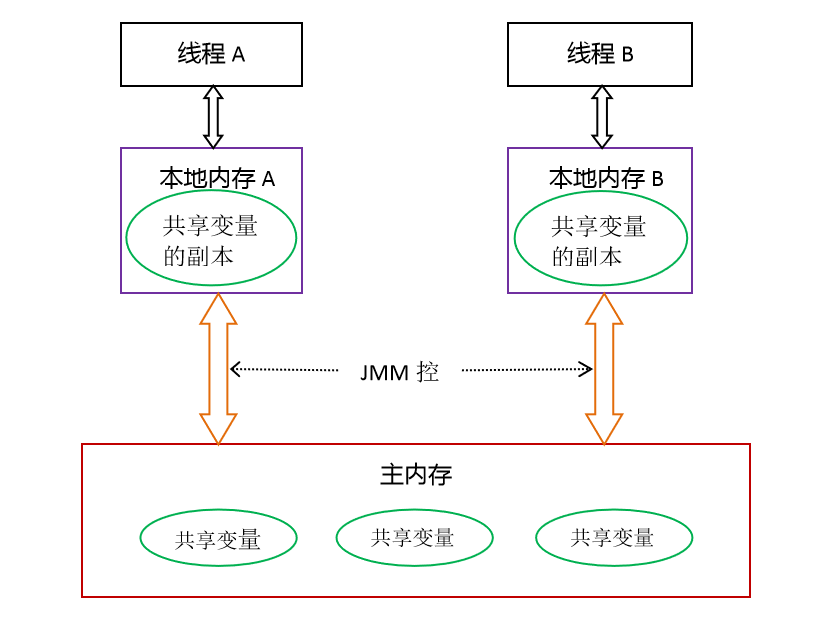
\includegraphics[width=0.7\linewidth]{figures/JMM.png}
	\caption{}
	\label{fig:JMM}
\end{figure}
\subsubsection{Java内存模型中的可见性, 原子性和有序性}
可见性, volatile \par
原子性, 各种锁 \par
有序性, 线程内有序 \par
\subsubsection{happen-before原则}
虽然有好几个, 但基本上描述模糊的就不写了\par
(1) 锁的happen-before, 就是同一个锁的unlock操作happen-before此锁的lock操作. \par
(2) 传递性: A hb b, b hb c; A happen-before C; \par
(3) 对象的构造函数在finalize方法之前. 
\subsubsection{wait/notify, await/singal}
Condition 的 await,signal, singalAll 与 Object 的 wait, notify, notifyAll 都可以实现的需求,两者在使用上也是非常类似,都需要先获取某个锁之后才能调用,而不同的是 Object wait,notify 对应的是 synchronized 方式的锁,Condition await,singal 则对应的是 ReentrantLock (实现 Lock 接口的锁对象)对应的锁 \par
下方是Condition的示例
\subsubsection{多线程wait和sleep区别}
(1) 主要在获得执行权和释放锁之间的区别, wait会释放执行权, 然后释放锁 , sleep 只会释放执行权 \par
(2) 如果notifyAll() 如果有多个线程在等待, 只会有一个线程获得执行权. \par
\subsubsection{Collection<? extends Person> s}
这叫泛型上限, 这样取出都是按照上限类型来运算的. 不会出现安全隐患
\begin{lstlisting}
public class Message {
	/** 当前消息数量*/
	private int count = 0;
	/** 信息存放最大限数*/
	private int maximum = 20;
	/** 重入锁*/
	private Lock lock;
	/** 生产者锁控制器*/
	private Condition producerCondition;
	/** 消费者锁控制器*/
	private Condition consumerCondition;
	
	public Message() {}
	
	public Message(final Lock lock, final Condition producerCondition, final Condition consumerCondition) {
		this.lock = lock;
		this.producerCondition = producerCondition;
		this.consumerCondition = consumerCondition;
	}
	
	/**
	* 生产消息
	* */
	public void set() {
		/** 获取锁*/
		lock.lock();
		try {
			if (count <= maximum) {
				/** 生产一个消息*/
				System.out.println("生产者 线程" + Thread.currentThread().getName() + "生产了一个消息, 当前有" + (++count) + "个消息");
				/** 唤醒等待的消费者*/
				consumerCondition.signal();
			} else {
				try {
					/**
					* 如果当前消息大于 maximum信息最大数
					* 生产者进入睡眠/等待状态
					* */
					producerCondition.await();
					System.out.println("生产者 线程" + Thread.currentThread().getName() + "进入睡眠");
				} catch (InterruptedException e) {
					e.printStackTrace();
				}
			}
		} finally {
			/** 释放锁*/
			lock.unlock();
		}
	}
	
	/**
	* 消费消息
	* */
	public void get() {
		/** 获取锁*/
		lock.lock();
		try {
			if (count > 0) {
				/** 消费一个消息*/
				System.out.println("消费者 线程" + Thread.currentThread().getName() + "消费了一个消息, 当前有" + (--count) + "个消息");
				/** 唤醒等待的生产者*/
				producerCondition.signal();
			} else {
				try {
					/** 如果没有消息, 消费者进入睡眠/等待状态*/
					consumerCondition.await();
					System.out.println("消费者 线程" + Thread.currentThread().getName() + "进入睡眠");
				} catch (InterruptedException e) {
					e.printStackTrace();
				}
			}
		} finally {
			/** 释放锁*/
			lock.unlock();
		}
	}
	
}

public class Producer implements Runnable {
	private Message message;
	public Producer(Message message) {
		this.message = message;
	}
	
	@Override
	public void run() {
		while(true) {
			try {
				Thread.sleep(500);
			} catch (InterruptedException e) {
				e.printStackTrace();
			}
			message.set();
		}
	}
	
}
public class Consumer implements Runnable {
	private Message message;
	public Consumer(Message message) {
		this.message = message;
	}
	
	@Override
	public void run() {
		while(true) {
			try {
				Thread.sleep(1000);
			} catch (InterruptedException e) {
				e.printStackTrace();
			}
			message.get();
		}
	}
	
}
import java.util.concurrent.locks.Condition;
import java.util.concurrent.locks.Lock;
import java.util.concurrent.locks.ReentrantLock;

public class App {
	public static void main(String[] args) {
		/** 重入锁*/
		final Lock lock = new ReentrantLock();
		/** 生产者锁控制器*/
		final Condition producerCondition = lock.newCondition();
		/** 消费者锁控制器*/
		final Condition consumerCondition = lock.newCondition();
		final Message message = new Message(lock, producerCondition, consumerCondition);
		/** 建几个生产线程*/
		new Thread(new Producer(message)).start();
		new Thread(new Producer(message)).start();
		new Thread(new Producer(message)).start();
		/** 建几个消费线程*/
		new Thread(new Consumer(message)).start();
		new Thread(new Consumer(message)).start();
		new Thread(new Consumer(message)).start();
		new Thread(new Consumer(message)).start();
	}
	
}


\end{lstlisting}
\subsubsection{线程的状态有哪些?}
(1) 新建状态(NEW): 线程创建之后 \par
(2) 可运行(RUNNING): 可能正在运行, 也可能正在等待时间片 \par
(3) 阻塞(BLOCKED): 等待获取一个排它锁, 如果期限陈释放了锁就会结束此状态. \par
(4) 无线等待(WAITING): 等待其他线程显式地唤醒, 否则不会被分配CPU时间片片 \par
(5) 限期等待(TIME\_WAITING): 如果没人唤醒在一定时间内系统会自动唤醒 \par
(6) 终止(TERMINATED): 可以是线程结束任务之后自己结束, 或者产生了异常而结束 \par
线程创建之后处于New状态, 调用start()方法后开始运行, 线程这时候处于Ready可运行状态. 可运行状态的线程获得cpu时间片后就处于RUNNING状态. 当线程执行wait()方法之后, 线程进入WAITING(等待)状态. 进入等待状态的线程需要依靠其他线程的通知才能够返回到运行状态, 而TIME\_WAITING超时等待状态相当于在等待状态的基础上增加了超时限制, 比如通过SLEEP方法或wait放假将java线程至于TIME\_WAITING状态, 到超时之后, java线程将会发挥RUNNABLE状态. 当线程调用同步方法是,在没有获取到所的情况下,线程将会进入到BLOCK状态. 执行完Runnable的run()方法之后将会进入到TERMINATED状态.
\begin{figure}
	\centering
	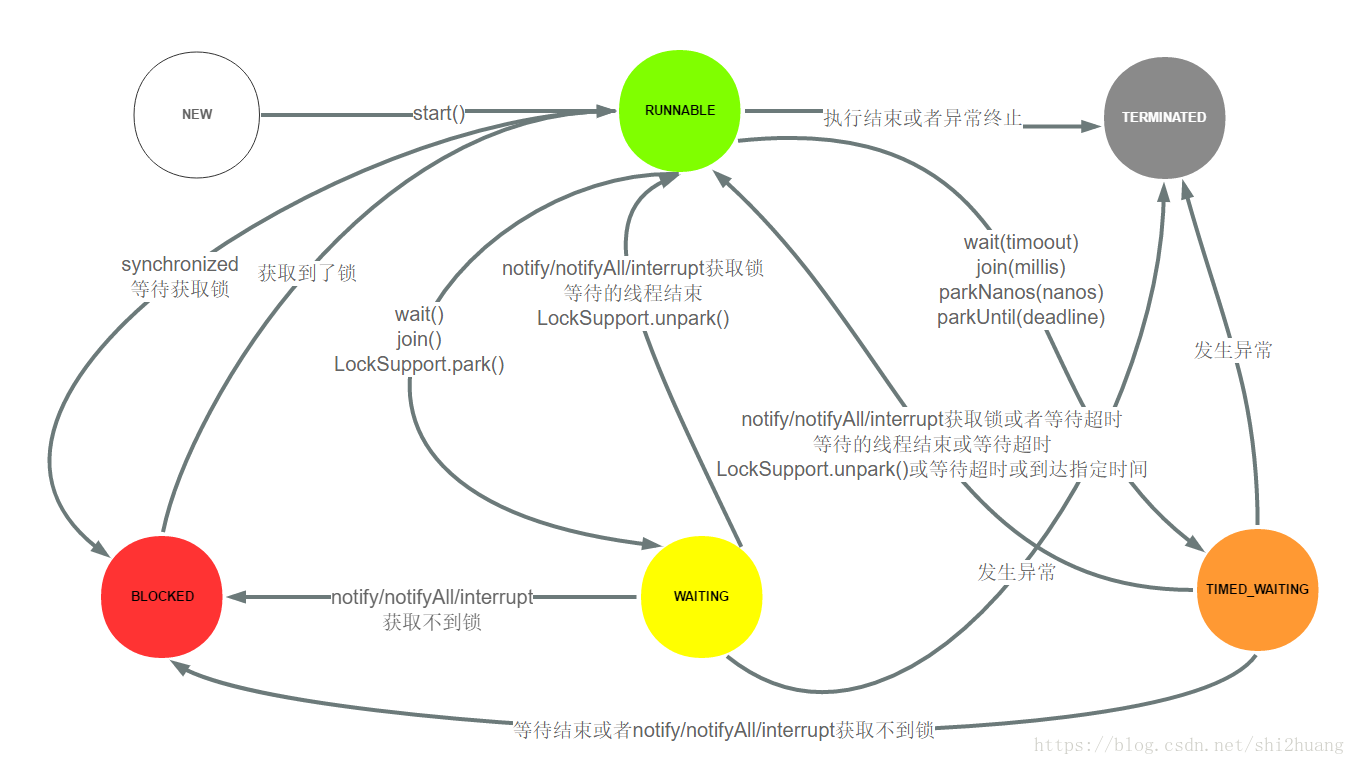
\includegraphics[width=0.7\linewidth]{figures/javaThreadState.png}
	\caption{}
	\label{fig:javaThreadState}
\end{figure}
\subsubsection{创建线程的几种方式}
(1) 继承Thread类创建线程 \par
定义Thread类的子类, 并重写该类的run方法\par
创建实例\par
调用实例start()方法 \par
(2) 实现Runnable接口创建线程 \par
实现一个接口类, 重新run方法. \par
创建Runnable实现类实例, 并以此实例作为Thread的target来创建Thread对象, 该Thread对象才是真正的线程对象. \par
调用线程对象start方法来启动该线程\par
(3) 使用Callable和Future创建线程: 与Runnable相比Callable是有返回值的, 返回值通过FutureTask进行封装 \par
创建Callable接口的实现类, 并实现call()方法, 该call()方法将作为线程执行体, 兵器有返回值 \par
创建Callbale实现类实例, 使用FutureTask类来包装Callable对象, 该FutureTask对象封装了该Callable对象的call()方法的返回值. \par
使用FutureTask对象作为Thread对象的target创建biang启动新线程\par
调用FutureTask对象的get()方法来获得子线程执行结束后的返回值 \par
(4) 使用线程池例如Executor框架(工厂方法) \par
(5) 创建线程的方式的对比\par
1. Runnable 不可以抛出异常, Callable可以 \par
2. Runnable 不可以有返回值, Callable 通过封装FutureTask 可以拿到返回值 \par
\subsubsection{synchronized锁升级: 无锁, 偏向锁, 轻量级锁, 重量级锁(与锁的优化一起学习}
这个叫做锁的膨胀. \par
(1) 偏向锁, 初次执行到synchronized代码块的时候, 锁对象变成偏向锁, 通过CAS修改对象投里的锁标志位, 字面意思是"偏向于第一个获得它的线程"的锁. 会存储获取锁的线程的地址. 偏向锁解锁, 不需要修改对象头的markword, 减少了一次CAS操作, 锁不会释放, 但是遇到冲突, 会由JVM来进行判断升级. 执行完同步代码块之后, 线程并不会主动释放偏向锁, 当第二次达到同步代码块时, 线程会判断此时持有锁的线程是否就是自己(持有锁的线程ID也在对象头里), 如果是正常往下执行. 由于之前没有释放锁, 这里也就不需要重新加锁. 如果自始至终使用锁的线程只有一个, 很明显偏向锁几乎没有额外开销, 性能极高. \par
(2) 轻量级锁, 自旋锁, 地担忧第二个线程加入锁竞争, 偏向锁, 就升级为轻量级锁. 只有当某线程获取锁的时候, 发现该锁已经被占用, 只能等待其实方, 这才发生了锁的竞争. 在所竞争下, 没有抢到锁的线程将自旋, 即不停的循环判断锁是否能够被成功获取. 长时间的自选操作是非常消耗资源的, 一个线程持有锁, 其他线程就只能在原地空号CPU. 如果达到某个最大自旋次数, 会将轻量级锁升级为重量级锁. 当后续线程尝试获取锁时, 直接将自己挂起.\par
(3) 偏向锁, 假定条件只有一个线程去获取锁 \par
(4) 轻量级锁, 假定条件是 多个线程交替去获取锁 \par
\subsubsection{如何使用synchronized}
1. 普通同步方法

\section{JVM}
%\subsection{二级标题}
\subsubsection{说一下JVM中, 哪些是共享区, 哪些可以作为gc root}
共享区: 方发区和堆 \par
每个线程独有: 栈, 本地方法栈, 程序技术器 \par
堆中, 从gc root可以找到一连串的对象, 就是正常的对象, 没有被找到的对象可以被回收.
\subsubsection{你们项目如何排查JVM问题}
1. 使用jvisualvm图形化查看内存的变化, 发现频繁的fullgc, 但是并没有出现oom现象, 可能是年轻代的内存不够, 对于大对象如果新生代放不下会直接放入老年代, 导致频繁fullgc, 通过增大新生代内存, fullgc减少, 证明修改有效. \par
2. 对于已经发生了oom异常的, 生成dump文件(-XX:+HeapDumpOnOutOfMemoryError -XX:HeapDumpPath=/usr/local/base) \par
使用jvisualvm等工具来分析dump文件, 更具dump文件找到异常的实例对象, 和异常的线程, 定位到具体的代码, 然后再进行详细的分析和调试 \par
\subsubsection{GC的三种收集方法: 标记清除, 标记整理, 复制算法的原理与特点, 分别用在什么地方, 如果让你优化收集方法, 有什么思路}
\begin{enumerate}
	\item 标记清除: 先标记, 标记完毕之后再清除, 缺点: 效率不高会产生碎片.
	\begin{figure}
		\centering
		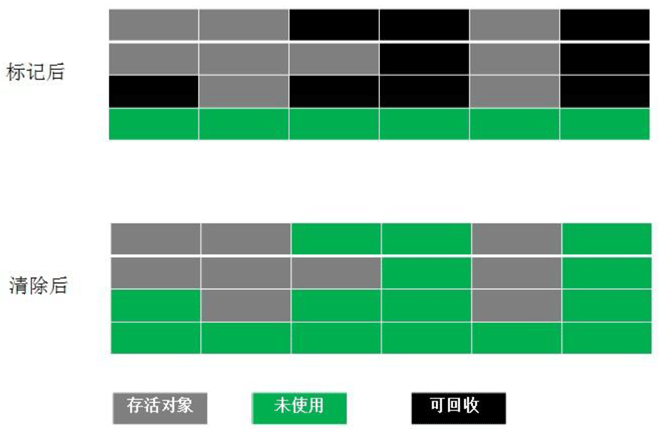
\includegraphics[width=0.7\linewidth]{figures/sign_remove.png}
		\caption{}
		\label{fig:sign_remove}
	\end{figure}
	\item 标记整理: 标记完毕之后, 让所有存活的对象向一端移动
	\item 复制算法: 分别8:1的Eden去和survivor区
	\begin{figure}
		\centering
		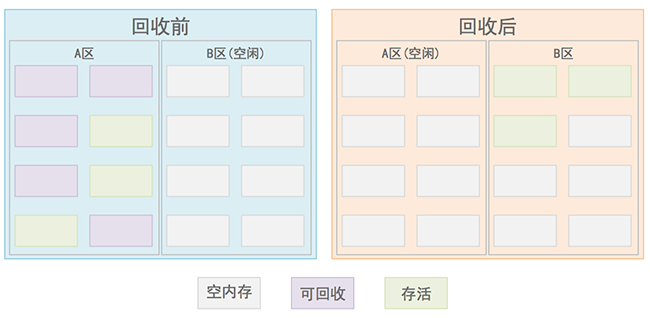
\includegraphics[width=0.7\linewidth]{figures/jvm_copy.jpg}
		\caption{}
		\label{fig:jvm_copy}
	\end{figure}
	\item 分代收集算法-重点 \par
	一般将Java分成新生代和老年代, 新生代使用复制算法, 老年代使用标记整理算法.
\end{enumerate}
\subsubsection{JVM的主要组成部分及其作用?}
JVM包含两个子系统和两个组件, 两个子系统为Class loader(类加载), Execution engin(执行引擎); 两个组件为 Runtime data area(运行时数据区), native Interface(本地接口)

\begin{enumerate}
	\item Class loader: 根据给定的额全限定类名(如:java.lang.object)来装在class文件到Runtime data area中的method area.
	\item Execution engine(执行引擎): 执行classes中的指令
	\item native Interface(本地接口): 与native libraries交互, 是其他编程语言交互的接口.
	\item Runtime data area(运行时数据区): 这就是我们常说的jvm的内存
\end{enumerate}
\par
\textbf{作用:} 首先通过编译器吧java代码转换成字节码, 类加载器(ClassLoader) 再把字节码加载到内存中, 将其放在运行时数据区(Runtime data area)的方发区内, 而字节码文件知识jvm的一套指令集规范, 并不能直接交给底层操作系统去执行, 因此需要特定的命令解析器执行引擎(Execution Engine), 将字节码翻译成底层系统指令, 在交由CPU去执行, 而这个过程中需要调用其他语言的本地库接口(Native Interface) 来实现整个程序的功能. 
\par
Java程序运行机制步骤
\begin{enumerate}
	\item 编码: IDEA等IDE进行编码java, 后缀.java
	\item 编译: javac 将源代码编译成字节码文件,字节码文件的后缀名为.class
\end{enumerate}
类的加载是将类的.class文件中的二进制数据读入到内存中, 将其放在运行时数据区的方法去内, 然后在堆区创建一个java.lang.Class对象, 用来封装类在方区内的数据结构.
\subsubsection{JVM运行时数据区}
运行时数据区由如下几个区域构成
\begin{enumerate}
	\item 程序计数器(PC): 当前线程所执行字节码的行号指示器, 字节码解析器的工作是通过改变这个计数器的值, 来选去下一条需要执行的字节码指令.
	\item java虚拟机栈(Java Virtual Machine Stacks): 用于存储局部变量表, 操作数栈, 动态链接, 方法出口等信息.
	\item 本地方法栈(Native Method Stack) : 与虚拟机栈的作用是一样的, 只不过虚拟机栈是服务Java方法的, 而本地方法栈是为虚拟机调用Native方法服务的.
	\item Java堆(Java Heap): Java 虚拟机中内存最大的一块, 是被所有线程共享的, 几乎所有的对象实例, 都在这里分配内存;
	\item 方法区(Method Area): 用于存储已被虚拟机加载的类信息, 常量, 静态变量, 及时编译后的代码等数据.
\end{enumerate}
\begin{figure}
	\centering
	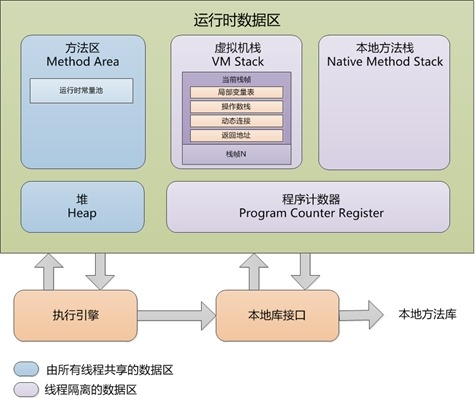
\includegraphics[width=0.7\linewidth]{figures/jvm.jpg}
	\caption{}
	\label{fig:jvm}
\end{figure}
\subsubsection{JVM运行时数据区这些方法的关系}
\begin{figure}
	\centering
	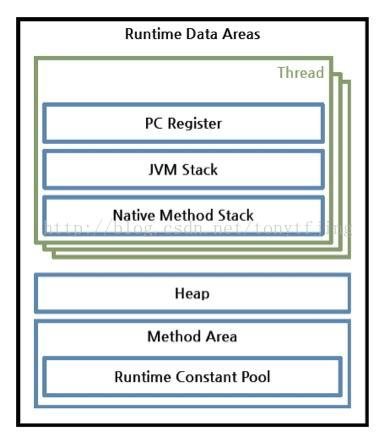
\includegraphics[width=0.7\linewidth]{figures/jvmRunTime.jpg}
	\caption{}
	\label{fig:jvmRunTime}
\end{figure}
可以看到PC指针和虚拟机栈和本地方法栈是线程独有的. 而堆,方法区和运行时常量池是属于线程共享
\subsubsection{永久代PermGen 和 元空间Metaspace 区别}
\begin{enumerate}
	\item 永久代PermGen : 是jdk1.7 对于方发区的实现. 由于动态生成类的情况比较容易出现永久代的内存溢出, 抛出异常. 而且字符串存储在永久代中容易出现性能问题和内存溢出.
	\item 元空间MetaSpace: 存在于本地内存.
\end{enumerate}
\subsubsection{说一下堆栈的区别?}
\textbf{物理地址}
\par
堆的物理地址分配对对象是不连续的. 因此, 性能慢些. 在GC的时候也要考虑到不连续的分配, 所以后各种算法. 比如, 标记-清除, 复制, 标记压缩, 分代(即新生代生活复制算法, 老年代使用标记压缩算法);
\par
栈使用的是数据结构中的栈, 先进后出的原则, 物理地址分配是连续的. 所以性能快.
\par
\textbf{内存区别}
\par
堆因为是不连续的, 所以分配的内存是在\textbf{运行期}确认的, 因此大小不固定. 一般堆大小远大于栈.
\par
栈是连续的, 所以分配的内存大小要在编译器就确认, 大小是固定的.
\par
\textbf{程序的可见度}
\par
堆对于整个应用程序都是共享, 可见的.
栈只对于线程是可见的. 所以也是线程私有. 他的生命周期和线程相同.
TIPS:
\begin{enumerate}
	\item 静态变量放在方法区.
	\item 静态的对象还是放在堆.
\end{enumerate}
\subsubsection{常见的垃圾收集器?}
(1) Serial收集器, 单线程收集器, 会stop the word. \par
\begin{figure}
	\centering
	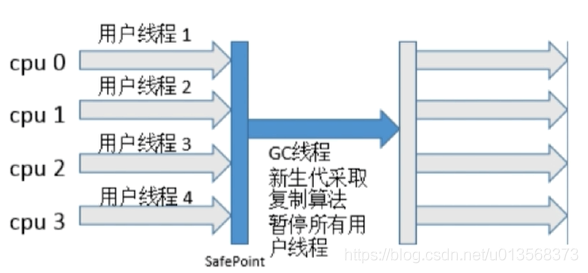
\includegraphics[width=0.7\linewidth]{figures/Serial.png}
	\caption{}
	\label{fig:Serial}
\end{figure}
(2) ParNew(Parallel Old)收集器, 是Serial收集器的多线程版本. 然后, 并行收集垃圾工作, 此时用户线程也是停止的状态 \par
\begin{figure}
	\centering
	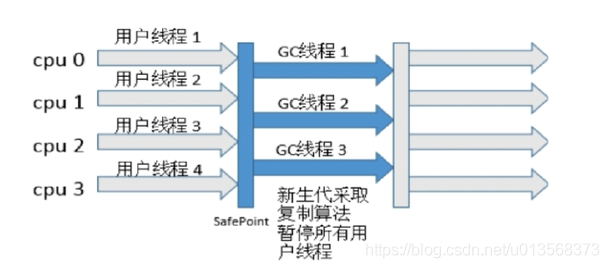
\includegraphics[width=0.7\linewidth]{figures/ParNew.png}
	\caption{}
	\label{fig:ParNew}
\end{figure}
(3) Parallel Scavenge 收集器(新生代) \par
多线程收集器, 同样是针对新生代. 停顿时间较短 \par
\begin{figure}
	\centering
	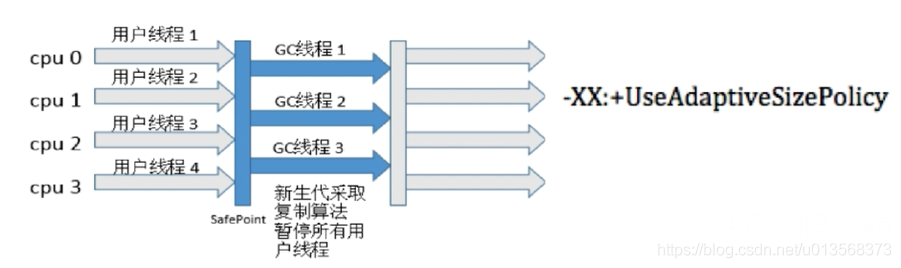
\includegraphics[width=0.7\linewidth]{figures/parallelscavenge.png}
	\caption{}
	\label{fig:parallelscavenge}
\end{figure}
(4) Serial Old 收集器(老年代) \par
使用标记整理算法收集老年代垃圾, 单线程. \par
(5) Parallel old 收集器(老年代) \par
标记整理算法, 多线程 \par
(6) CMS收集器 \par
简单来说, 在垃圾回收线程几乎能做到与用户线程同时工作, 使用标记清除算法. 
\begin{figure}
	\centering
	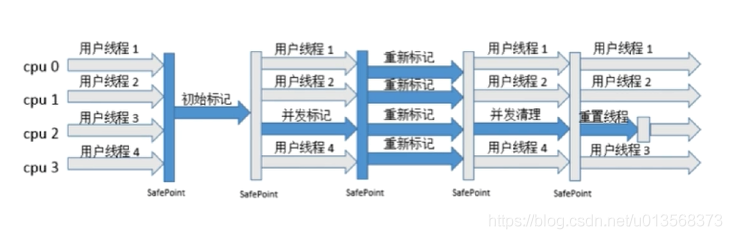
\includegraphics[width=0.7\linewidth]{figures/cms.png}
	\caption{}
	\label{fig:cms}
\end{figure}
(7) G1 收集器 \par
使用复制 + 标记 - 整理算法 收集新生代和老年代垃圾. 
\subsubsection{内存分配与回收策略. }
1. MinorGC 和 Full GC 有什么不同? \par
MINORGC: 新生代垃圾回收, 回收速度一般较快 \par
MajorGC: 老年代GC, 回收速度较慢 \par
FULLGC: 重GC, 会清理整个空间包括年轻代和老年代. \par
2. 什么时候对象进入老年代 \par
(1) 大对象直接进入老年代 \par
(2) 空间分配担保: 当TO被填满后 当其中的对象还村或者, 剩下的对象直接存入老年代 \par
(3) 年龄判定: 如果Survivor空间中相同年龄多有对象大小的总和大于Survivor空间的一半, 年龄大于或等于改年龄的对象就可以直接进入老年代, 如需达到要求的年龄 \par
\subsubsection{虚拟机性能监控和故障处理工具}
jvisualvm 可视化监控.
\subsubsection{简述JVM中类加载机制}
类加载过程: 加载, 验证, 准备, 解析和初始化. \par
(1) 加载 \par
1. 通过类的全限定名获取此类的二进制字节流 \par
2. 将这个字节流所代表的的静态存储结构转化为方发区的运行时数据结构 \par
3. 在内存中生成一个代表这个类的java.lang.Class对象, 作为方发渠这个类的各种数据的访问入口 \par
(2) 验证 \par
为了却表Class文件的字节流中包含的信息符合当前的虚拟机的要求, 并且不会危害虚拟机自身的安全. \par
(3) 准备 \par
正式为类变量(static修饰的)分配内存并设置类变量初始值的节点, 这些变量所使用的的内存都将在\textbf{方法区}中进行分配 \par
(4) 解析 \par
虚拟机将常量池内的符号引用替换为直接引用的过程. 主要对类过接口, 字段, 类方法, 接口方法的解析, 主要是静态链接, 方法主要是静态方法和私有方法. \par
\subsubsection{对象的访问定位?}
目前主流的访问方式有句柄和直接指针两种方式.

\begin{enumerate}
	\item 指针: 指向对象, 代表一个对象再内存中的起始地址
	\item 句柄: 可以理解为指向指针的指针, 维护者对象的地址. 句柄不直接指向对象, 而是指向对象的地址(句柄不发生变化, 指向固定内存你地址), 再由对象的指针指向对象的真实内存地址.
\end{enumerate}
\textbf{句柄访问}
\par
Java堆中划分出一块内存作为句柄池, 引用中存储对象的句柄地址, 而句柄中包含了\textbf{对象实例数据}与\textbf{对象类型数据}各自的决堤地址信息, 具体构造如下图所示:
\begin{figure}
	\centering
	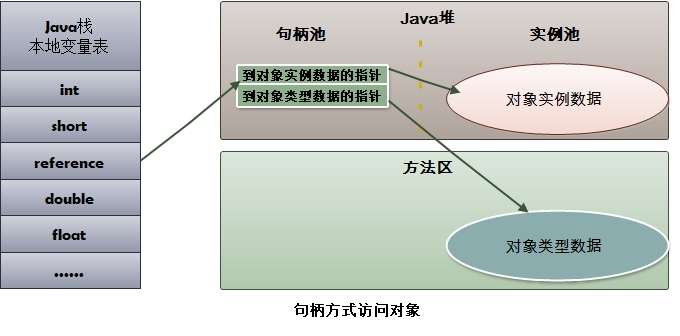
\includegraphics[width=0.7\linewidth]{figures/jvm_handler.jpg}
	\caption{}
	\label{fig:jvm_handler}
\end{figure}
\textbf{直接指针}
\par
\begin{figure}
	\centering
	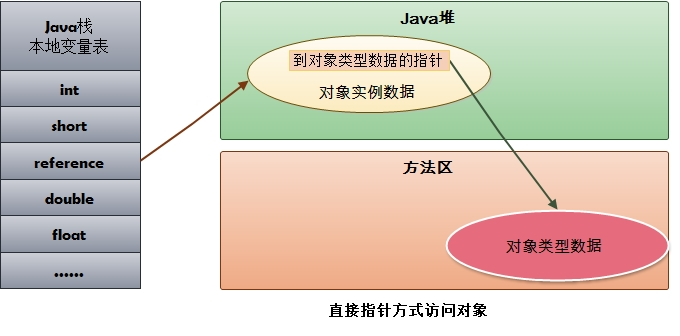
\includegraphics[width=0.7\linewidth]{figures/jvm_point.jpg}
	\caption{}
	\label{fig:jvm_point}
\end{figure}
\subsubsection{垃圾回收器的基本原理是什么?}
\textbf{可达性分析}
\par
GC采用有向图的方式记录和管理堆中的所有对象. 通过这种方式确定哪些对象是"可达的", 哪些对象是"不可达的", 当GC确定一些对象为"不可达"时, GC就有责任回收这些内存空间.
程序员可以手动执行System.gc(), 通知GC运行, 但是Java语言规范并不保证GC一定会执行.
\par
\textbf{引用计数法}
为每个对象创建一个引用技术, 有对象引用时计数器+1, 引用被释放是技术-1, 当计数器为0时就可以被回收. 优缺点, 不能解决循环引用的问题.
\subsubsection{在java中, 对象什么时候可以被垃圾回收?}
当对象变的不可触及的时候, 这个对象就可以被回收了, 垃圾回收不会发生在永久代, 如果永久代满了或者是超过了临界值, 会触发完全垃圾回收(full gc), 会导致Stop-the-world. 
\subsubsection{如何判断对象已经死亡?}
(1) 引用计数法, 标记为零. 缺点难以解决互相引用问题 \par
(2) 可达性分析, 当一个对象到GC Root对象没有任何路径可达. \par
(3) 上面两种都是暂时处于缓刑阶段, 真正宣告一个对象死亡, 至少要经历两次标记过程.
\subsubsection{简述强, 软, 弱, 虚引用?}
(1) 强引用 \par
如果一个对象具有强引用, 垃圾回收期绝不会回收它 \par
(2) 软引用(SoftRef) \par
如果内存足够, 垃圾回收期就不会回收塔, 如果内存不足了, 就会回收这些对象的内存. 可以实现内存敏感的告诉缓存. \par
(3) 弱引用(WeakRef) \par
弱引用关联的对象只能生存到下一次垃圾回收之前. \par
(4) 虚引用(ReferenceQue) \par
如果一个对象仅持有虚引用, 那么他就和没有任何引用一样, 在任何时候都可能被垃圾回收. 必须和引用队列一起联合使用.\par
\textbf{区别:} \par
软弱引用都是发生在垃圾回收动作之后, 虚引用发生在垃圾回收动作之前.



\section{Redis}
%\subsection{二级标题}
\subsubsection{Redis的数据结构及使用场景}
字符串(string), 用来缓存简单的数据结构, 简单的字符串, 可以实现Session共享\par
列表(list), Redis的列表通过命令的组合, 即可以当做栈, 也可以当做队列来使用\par
集合(set), 可以实现自己和某人共同关注的人\par
散列表(hash), 存储一些key-value对, 更适合用来存储对象\par
有序集合(sorted set). 设置顺序, 实现排行榜的功能\par
\subsubsection{Redis集群策略}
一主多从, 整个集群所能存储的数据收到某台机器的内存容量, 所以不可能支持特大数据量, 一般加上哨兵模式来使用 \par
Cluster模式: 槽分配. 支持多主多从

\subsubsection{什么是Redis?}
\begin{enumerate}
	\item 高性能非关系型数据库
	\item 可以存储五种不同类型的额值之间的映射. 键的类型只能为字符串, 值支持五种类型数据:字符串(string), 列表(list), 集合(set), 散列表(hash), 有序集合(sorted set).
	\item redis数据是存在内存中的, 所以读写速度非常快.
\end{enumerate}
\subsubsection{简述Redis单线程模型?}
实现方式
\par
(1) I/O多路复用
\par
简单来说, 可以使用I/O多路复用来坚定多个socket连接, 然后将感兴趣的时间注册到内核中并监听每个事件是否发生. 
\par
(2) 基于事件驱动
\par
服务器需要处理两类事件, 文件事件; 时间事件.
\par
当被监听的套接字准备好执行连接应答(accept), 读取(read), 写入(write), 关闭(close)等操作时, 与操作相对应的文件事件就会产生, 这时文件事件处理器就会调用套接字之前关联好的事件处理器来处理这些事件.
\par
文件事件处理器(file event handler) 主要包含4个部分: 多个socket(客户端链接), IO多路复用, 文件事件分派; 事件处理;
\begin{figure}
	\centering
	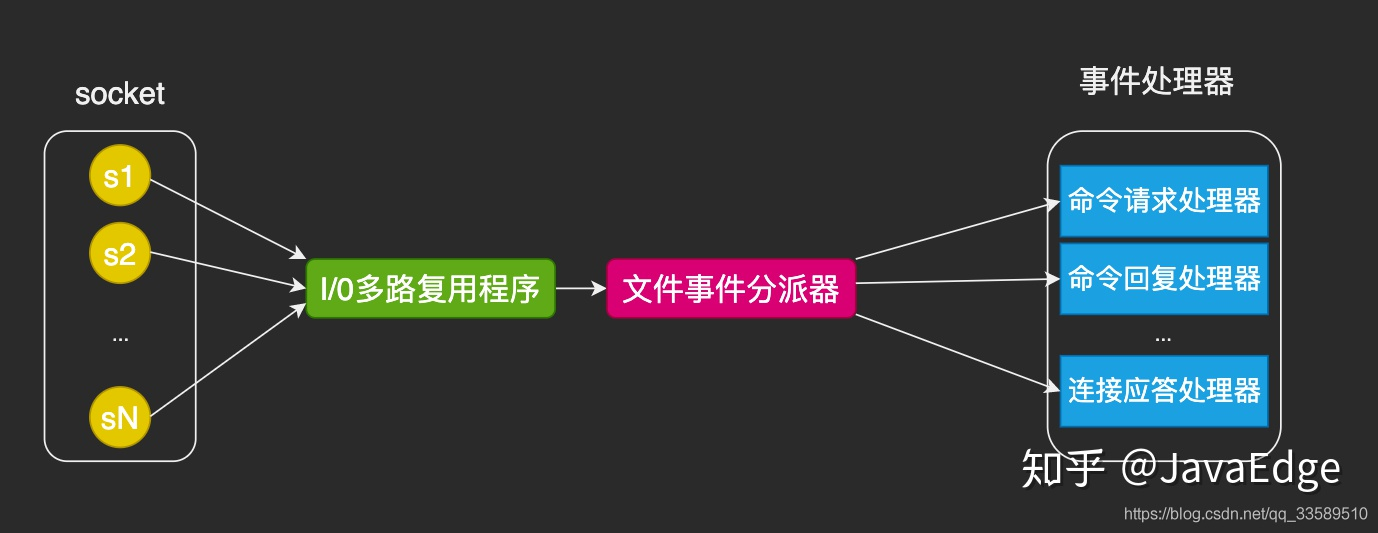
\includegraphics[width=0.7\linewidth]{figures/redis_file_event.jpg}
	\caption{}
	\label{fig:redis_file_event}
\end{figure}
\subsubsection{Redis五种类型数据的实现方式}
\begin{table}[!htbp]
	\centering
	\caption{实现}
	\begin{tabular}{|l|r|}
		
		\hline
		类型&编码\\
		\hline
		STRING&INT(整形, 在String中存储整形会是的)\\
		\hline
		STRING&EMBSTR(简单动态字符串, 对于短小的string(44位字符)会使用这种结构)\\
		\hline
		STRING&RAW(简单动态字符串, 对于稍微长一点的string会使用(44位字符)这种结构)\\
		\hline
		LIST&QUICKLIST(快表)\\
		\hline
		LIST&LINKEDLIST(快表)\\
		\hline
		SET&INTSET(整数集合)\\
		\hline
		SET&HT(哈希表)\\
		\hline
		ZSET&ZIPLIST(压缩列表)\\
		\hline
		ZSET&SKIPLIST(跳表)\\
		\hline
		HASH&ZIPLIST(压缩列表)\\
		\hline
		HASH&HT(哈希表)\\
		\hline
	\end{tabular}
\end{table}
字符串结构SDS和C中char[]有什么不同
\begin{enumerate}
	\item 获取SDS中字符串的长度因为SDS中存储了字符串的长度len属性, 直接访问, 时间复杂度O(1), 对于C语言获取字符串的长度需要经过遍历, 时间复杂度O(n).
	\item 避免缓冲区溢出, 会检查SDS中属性, free(空闲空间)能够实现字符串的扩充判断. 不足会重新申请空间.
	\item SDS支持空间预分配, 扩展的内存比实际需要的多
	\item SDS支持空间惰性释放, 字符串缩短之后, 不立即进行空间回收操作. SDS也提供相应API, 可以对冗余空间进行回收.
	\item 可以存储二进制, 因为SDS不以回车符号进行终止的判定.
\end{enumerate}
\subsubsection{redis字典的底层实现hashTable相关问题}
\begin{enumerate}
	\item 解决冲突: 链地址法, 即使用数组+链表的方式实现. 
	\item 扩容: 有两个指针h[0] 和 h[1], h[1] 用来备份, 当h[0], 满了使用渐进值hash, 插入都插入h[1], 查找两个表都进行查找.
\end{enumerate}
\subsubsection{压缩链表原理ziplist}
连续内存, 包含多个节点entry.
\begin{figure}
	\centering
	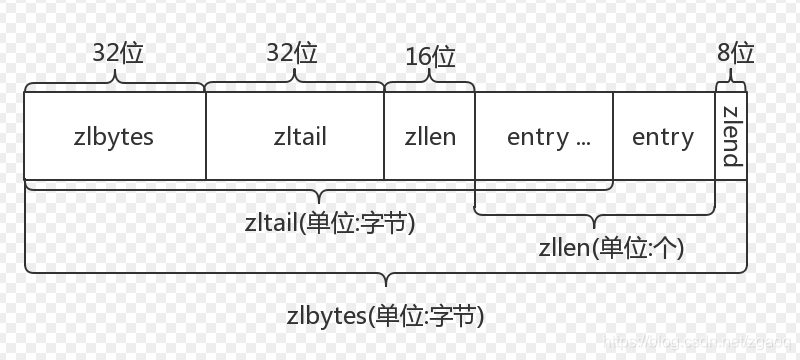
\includegraphics[width=0.7\linewidth]{figures/ziplist.png}
	\caption{}
	\label{fig:ziplist}
\end{figure}
\subsubsection{zset}
本质是舵机链表并有序.
skiplist与平衡树, 哈希表的比较
\begin{enumerate}
	\item skiplist和各种平衡树的元素排序是有序 的, 而哈希表不是有序的, 因此, 在哈希表上智能做单个key的查找, 不适宜做范围查找.
	\item 在做范围查找的时候, 平衡树比skiplist操作要复杂. 在平衡树上, 需要做一步回退操作. 而在skiplist上进行范围查找就非常简单, 只要找到最小值之后对第一层链表进行若干部遍历就可以实现.
	\item 平衡树插入和删除操作, 会引起结构调整, 操作复杂, skiplist的插入和删除只需要修改相邻节点的指针, 操作简单又快速.
\end{enumerate}

\subsubsection{AOF和RDB两种持久化方式区别}
\begin{enumerate}
	\item AOF存储命令, RDB存储数据.
	\item AOF文件因为存储命令, 所以在redis启动的时候加载aof会比加载rdb要慢. 
	\item Redis 4.0 之后 启动了混合模式, AOF不需要是全量日志, 只要保存前一次RDB存储开始到这段时间增量AOF日志即可.
\end{enumerate}
\subsubsection{Redis中过期策略和缓存淘汰机制}
\begin{enumerate}
	\item 定期删除: redis默认每隔100ms随机对key检查, 有过期的key则进行删除. 容易导致很多过期的key没被发现
	\item 惰性删除: 获取某个key的时候, redis会检查一下, 如果过期了就进行删除.
\end{enumerate}
\subsubsection{为什么要使用Redis}
\begin{enumerate}
	\item 高性能: 内存的读取比硬盘乃至固态硬盘的读取速度都要快得多
	\item 高并发: 直接操作缓存能够承受的请求是远远大于直接访问数据库的, 所以我们可以考虑把数据库中的部分数据转移到缓存中去, 这样用户的一部分请求会直接请求缓存这里而不用经过数据库. 
	\item 高性能: 使用多路I/O复用木星, 非阻塞IO;
\end{enumerate}
\subsubsection{Redis底层实现跳表介绍一下}
跳表是带多级索引的链表, 时间复杂度O(lgn), 所能实现的功能和红黑树差不多, 但是跳表有一个区间查找的优势, 红黑树没有.
\begin{figure}
	\centering
	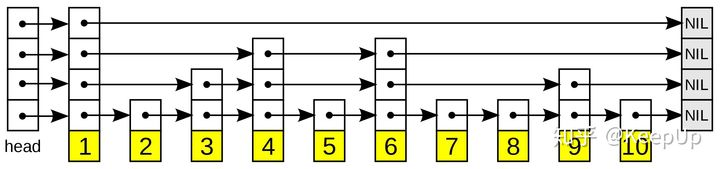
\includegraphics[width=0.7\linewidth]{figures/jump_table.jpg}
	\caption{}
	\label{fig:redissharding}
\end{figure}
\begin{enumerate}
	\item 表头: 负责维护跳表的节点指针.
	\item 跳跃表节点: 保存着元素值, 以及多个层.
	\item 层: 保存着指向其他元素的指针, 高层的指针越过的元素数量大于等于底层的指针, 为了提高查找效率, 程序总是从高层先开始访问, 然后随着元素值范围的缩小, 慢慢降低层次.
	\item 表尾: 全部由NULL组成.
\end{enumerate}

\subsubsection{为什么要使用Redis而不用map/guavaCache做缓存}
\begin{enumerate}
	\item guavaCache实现的是本地缓存, 最主要的特点是轻量化以及快速, 生命周期随着jvm的销毁而结束, 冰洁在多实例的情况下, 每个实例都需要个字保存一份缓存, 缓存容易出现不一致性.
	\item 使用redis之类的缓存称为分布式缓存, 在多实例的情况下, 各实例公用一份缓存数据, 缓存具有一致性.
\end{enumerate}
\subsubsection{分布式锁如何使用redis实现}
\begin{enumerate}
	\item setnx命令原子性实现. 
\end{enumerate}
\subsubsection{Redis的内存淘汰策略有哪些}
Redis的内存淘汰策略是指在Redis用于缓存的内存不足时, 怎么处理需要新写入且需要申额外空间的数据.
全局的键空间选择性移除
\begin{enumerate}
	
	\item noeviction: 当内存不足以容纳新写入数据时, 新写入操作会报错.
	\item allkeys-lru: 当内存不足以容纳新写入数据时, 在键空间中, 移除最近最少使用的key.
	\item allkeys-random: 当内存不足以容纳新写入数据时, 在键空间随机移除某个key.
\end{enumerate}
设置过期时间的键空间选择性移除
\begin{enumerate}
	
	\item volatile-lru: 当内存不足以容纳新写入数据时, 在设置了过期时间的键空间中, 移除最近最少使用的key.
	\item volatile-random: 当内存不足以容纳新写入数据时, 在设置了过期时间的键空间中, 随机移除某个key.
	\item volatile-ttl: 当内存不足以容纳新写入的数据时, 在设置了过期时间的键空间中, 有更早过期时间的key优先移除. 
\end{enumerate}
\subsubsection{Redis事物的概念}
Redis事物的本质通过MULTI, EXEC, WATCH等一组命令的集合. 
\begin{enumerate}

	\item 事物开始 MULTI
	\item 命令入队
	\item 事务执行 EXEC
\end{enumerate}
* 事务执行过程中, 如果服务端收到有EXEC, DISCARD, WATCH, MULTI之外的请求, 将会把请求放入队列中排队.
简单介绍一下watch, 当watch的变量在事务过程中发生了改变, 那么事务失败, 拒绝执行事物.
\begin{lstlisting}
	>watch 'name'
	>multi
	>set "name" "peter"
	>exec
	(nil)
\end{lstlisting}
\subsubsection{RedisSharding}
简单来说就是多个client 连接多个redis, 然后通过一致性哈希算法, 来确定访问的key+访问的客户端名字在哪一台redis上.
采用的算法是MURMUR\_HASH, 
\begin{figure}
	\centering
	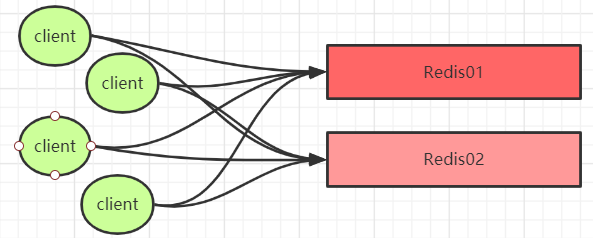
\includegraphics[width=0.7\linewidth]{figures/redis_sharding.png}
	\caption{}
	\label{fig:redissharding}
\end{figure}
\subsubsection{缓存雪崩}
缓存同一时间大面积的失效, 所以, 后面的请求都会落到数据库上, 造成数据库短时间内承受大量请求而崩掉

\par
\textbf{解决方案}
\begin{enumerate}
	
	\item 缓存数据的过期时间设置随机, 防止同一时间大量数据过期现象发生.

\end{enumerate}

\subsubsection{缓存穿透}
缓存和数据库中都没有数据, 导致所有的请求都落在数据库中, 造成数据库短时间内承受大量请求而崩掉.
\par
\textbf{解决方案}
\begin{enumerate}
	
	\item 从缓存中取不到的数据, 在数据库中也没有取到, 这时也可以将key-value对写为key-null, 缓存时间设定为30s.
	
\end{enumerate}

\subsubsection{缓存击穿}
缓存中没有但数据库中有的数据, 由于并发用户特别多, 同时读缓存没读到数据, 又同时去数据库取数据, 引起数据库压力瞬间增大, 造成过大压力, 和缓存雪崩不同的是, 缓存击穿指并发查询同一条数据, 缓存雪崩是不同数据都过期了, 很多数据都查不到, 从而查数据库.
\par
\textbf{解决方案}
\begin{enumerate}
	\item 设置热点数据永不过期	
\end{enumerate}
\subsubsection{缓存预热}
系统上线后, 将相关的缓存数据直接加载到缓存系统. 这样就可以避免在用户请求的时候, 先查询数据库, 然后再讲数据缓存的问题, 用户直接查询事先被预热的缓存数据.
\par
\textbf{解决方案}
\begin{enumerate}
	\item 定时刷新缓存;	
\end{enumerate}
\subsubsection{Redis6.0 为什么要引入多线程呢?}
Redis将所有数据放在内存中, 内存的相应市场大约100ns, 对于小数据包, Redis服务器可以处理8w到10wQPS, 这也是Redis处理的极限了, 对于80\%的公司来说, 单线程的redis已经足够使用了. 
\par
但随着越来越复杂的业务场景, 需要更大的QPS.
\begin{enumerate}
	\item 可以充分利用服务器CPU资源, 目前主线程只能利用一个核
	\item 多线程任务可以分摊Redis同步IO读写负荷.	
\end{enumerate}
\subsubsection{Redis主从复制模式}
\begin{enumerate}
	\item 完全同步:刚开始, 主服务器发送RDB文件给从服务器, 实现主从同步.
	\item 部分同步:当连接由于网络原因断开的时候, 将中间断开的执行的写命令发送给从服务器. 实现同步.	
\end{enumerate}
\subsubsection{Redis中持久化机制}
\begin{enumerate}
	\item 
\end{enumerate}


\section{计算机网络}
%\subsection{二级标题}
\subsubsection{计算机网络分层}
计算机网络OSI模型是七层, 如果是TCP/IP
应用层(HTTP/FTP) - 应用层
\par 
~ - 表示层
~ - 会话层
\par
传输层(UDP/TCP) - 传输层
\par
网际层(IP) - 网络层
\par 
主机至网络层 - 数据链路层
~ - 物理层
\subsubsection{TCP和UDP区别?}
\par
UDP: 面向报文, 支持1对1, 1对多, 多对1的交互通信
\par
TCP: 面向连接, 提供可靠交付, 有流量控制, 拥塞控制, 提供全双工通信, 面向字节流. TCP是点对点的.
\subsubsection{TCP三次握手相关问题}
为什么三次握手而不是两次握手: 主要是为了防止已失效的链接请求报文段突然又传送到了B, 因而产生错误. 如果只要两次握手就建立连接, 那么如果A第一次请求丢失了, A 又发送了一次请求, 但是这一次传输结束了, A上一次丢失的请求再次被传送到了B, 如果建立了连接, 但是A现在一直不回应B, 导致B浪费了资源.
\subsubsection{TCP四次挥手问题}
关闭连接的时候, 当Server端收到FIN报文时候, 很可能并不会立即关闭SOCKET, 所以只能先回复一个ACK报文, 告诉Client端, 你发送的FIN我收到了, 只有等我Server端所有的报文都发送完了, 我才能发送FIN报文. 不能一起发送, 所以需要四步挥手.
\subsubsection{TCP协议-如何保证传输的可靠性}
\textbf{超时重传:} 简单理解就是发送在发送完数据后等待一个时间, 时间到大没有接收到ACK报文, 那么对刚才发送的数据进行重新发送
\par
\textbf{连接管理:} 使用三次握手和四次挥手
\par
\textbf{流量控制:} TCP根据接收端对数据的处理能力, 决定发送端的发送速度, 这个机制就是流量控制. TCP协议的包头信息当中, 有一个16位字段的窗口大小, 发送方更具ACK报文里的窗口大小的值的改变自己的发送数据
\par
\textbf{拥塞控制:} 慢开始, 拥塞避免, 快重传, 快恢复.
\par
慢开始算法的思路就是, 不要一开始就发送大量的数据, 先探测一下网络的拥塞程度, 也就是说由小到大主键增加拥塞窗口的大小.
\par
拥塞避免算法让拥塞窗口缓慢增长, 即每经过一个往返时间RTT就把发送方的拥塞窗口cwnd加1, 而不是加倍. 这样拥塞窗口按线性归路缓慢增长.
\par
快重传和快恢复: 发送方只要一脸收到三个重复确认就引动立即重传对方尚未收到的报文段, 而不必继续等待设置的重传计时器时间到器.
\begin{figure}
	\centering
	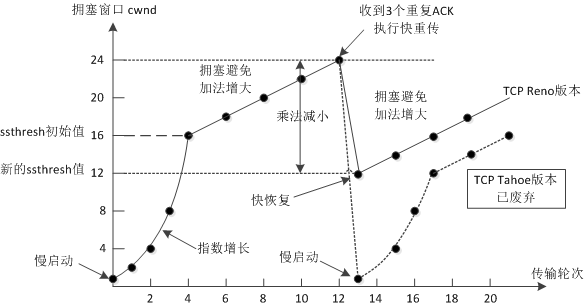
\includegraphics[width=0.7\linewidth]{figures/tcp.png}
	\caption{}
	\label{fig:tcp}
\end{figure}
\subsubsection{Cookie作用, 安全性问题和Session的比较}
(1) Cookie是服务器发送到用户浏览器并保存在本地的一小块数据,  他会在浏览器之后向统一服务器再次发送请求时被携带上.
\par
(2) Session 存储在服务器端. 使用Session维护用户登录状态的过程如下: (需要cookie作为传输机制)
用户进行登陆是, 用户提交包含用户名和密码的表单, 放入HTTP请求报文中;
服务器校验该用户名和密码, 如果正确则把用户信息存储到Redis中, 他在Redis中的key成为SessionId.
\par
服务器返回的响应报文Set-Cookie首部字段包含了这个SessionID, 客户端收到响应报文之后将该Cookie值存入浏览器中.客户端之后对同一个服务器进行请求时会包含该Cookie值, 服务器收到之后提取出SessionID, 从Redis中取出用户信息, 继续之前的业务操作.
\par
session 的运行依赖 session id, 而 session id 是存在 cookie 中的, 也就是,如果浏览器禁用了 cookie, 同时 session 也会失效(但是可以通过其它方式实现, 比如在 url 中传递 session\_id)
\par
cookie存在大小限制, 单个不超过4k, 浏览器中Cookie个数也有限制.
Session没有大小限制, 是和服务器内存有关的.
\subsubsection{HTTP1.1 和 HTTP1.0的比较}
HTTP1.1 默认长链接, 长连接只需要建立一次TCP连接, 进行多次HTTP通信.
HTTP1.0 默认短连接, 每进行一次HTTP通信就要新建一个TCP连接.
\subsubsection{HTTPS加密}
使用SSL连接. HTTPS采用混合加密算法, 使用非对称加密和对称加密, 非对称加密用于传输对称秘钥来保证传输过程的安全性, 之后使用对称秘钥加密进行通信来保证通信过程的效率. 
\par
HTTPS加密过程:
\begin{enumerate}
	\item 客户使用HTTPS的URL访问web服务器, 要求与Web服务器建立SSL链接.	
	\item Web服务器收到客户端请求后, 会将网站的证书信息(证书中包含公钥)传送一份给客户端.
	\item 客户端的浏览器与web服务器开始写上SSL链接的安全登记, 也就是信息加密登记.
	\item 客户端的浏览器更具双方同意的安全登记, 建立会话秘钥, 然后利用网站的公钥将会话秘钥加密, 并传送给网站
	\item Web服务器利用自己的私钥解密出会话秘钥.
	\item Web服务器利用会话秘钥加密与客户端之间的通信.
\end{enumerate}
\par
缺点: 因为需要进行加密解密等过程, 因此速度会更慢, 需要支付证书授权的高额费用.
\subsubsection{输入网址发生的事情}
\begin{enumerate}
	\item 浏览器查找该域名的IP地址
	\item 浏览器更具解析得到的IP地址向web服务器发送一个HTTP请求.
	\item 服务器收到请求并进行处理
	\item 服务器返回一个响应.
	\item 浏览器对该响应进行解码, 渲染显示.
	\item 页面显示完成后, 浏览器发送异步请求.
\end{enumerate}
\section{mysql}
%\subsection{二级标题}
\subsubsection{redo log 和 undo log, bin log }
如果修改直接修改到日志中的话, 性能开销比较大, mysql 会将要写的数据先写到redolog中,然后再讲redolog存储到磁盘中, 使用场景系统崩溃恢复 \par
bin log: 归档日志, 通过追加方式记录, 使用场景: 主从复制和数据恢复 \par
undo log: 回滚日志, MVCC多版本并发. 快照读是MVCC的一种体现方式.
\subsubsection{隔离级别}
\par
读已提交(read committed): 简单来说select * from account, 读出来的数据都是已经提交的数据.
\par 可以出现不可重复读(一个事物两次读到的事物不一样)和幻读(插入一条记录)
\par 
读未提交(read uncommitted) : 简单来说 select * from account, 读出来的数据是另一个事物还没有提交的数据, 
\par 可以出现脏读(无论是脏写还是脏读,都是因为一个事务去更新或者查询了另外一个还没提交的事务更新过的数据。因为另外一个事务还没提交,所以它随时可能会回滚,那么必然导致你更新的数据就没了,或者你之前查询到的数据就没了,这就是脏写和脏读两种场景。): 简单的说, 就是A事物在还没commit数据的情况下, b事物使用了A事物的数据, 但是A事物出现了回滚操作, 导致B事物读出来的数据是脏数据. 可以出现不可重复度, 可以出现幻读. (感觉是最不靠谱的一个级别)
\par 
可重复读(RR: Repeatable read) : 简单来说, 就是A事物插入了一条新数据, B事物没看到, 因为可重复读, 但是B是可以操作这条新数据的. 
\par 
串行化(serializable): 只能一个一个处理, 没什么问题, 但是效率太低一般不考虑.
\par 提示: 不可重复读对应的是修改即Update,幻读对应的是插入即Insert.
\par TIPS:
可见,幻读就是没有读到的记录,以为不存在,但其实是可以更新成功的,并且,更新成功后,再次读取,就出现了。
\subsubsection{ACID}
原子性: 不可分割
\par
一致性: 数据完整性, 例如金钱的综述
\par
隔离性: 不被打扰
\par
持久性: 永久保存
\subsubsection{乐观锁和悲观锁}
悲观锁, 指的是在整个数据处理过程中, 将数据处于锁定状态. 悲观锁的实现, 往往依靠数据库提供的锁机制.
\par
乐观锁的实现, 基于并发控制的CAS理论.
\subsubsection{MVCC}
MVCC用于提交读和可重复读这两种隔离级别. 使用undolog实现
\par
主要依靠事务版本号来实现读已提交和可重复读.
\par
当开始一个新事物时, 该事物的版本号肯定会大于当前所有数据行快照的创建的版本号
\subsubsection{RR和RC隔离级别下的InnoDB快照读有什么区别}
(1) RR隔离级别下, 当事物第一次进行快照读, 仅此一次创建read-view视图, 所以read-view
中未提交事物数组和最大事物ID始终保持不变, 因此每次读取时只会读取事物之前的数据 \par
(2) 而在RC隔离级别下, 每次事物进行快照读是, 都会生成新的read-view视图, 导致在RC隔离级别下事物可以看到其他事物修改后的数据, 这也是导致不可重复的原因 \par
总之, 在RC隔离级别下, 是每个快照读都会生成并获取最新的Read-View: 而在RR隔离级别下, 则是同一个事物中的第一个快照读才会创建Read View, 之后的快照读获取的都是同一个Read View \par
\subsubsection{B+/B树之间的比较}
(1) B+树空间利用率更高, 可减少IO次数. \par
(2) B+树所有关键字的查询路径长度相同(因为关键字在叶子节点), 导致每一次查询的效率相当, 更加稳定. \par
(3) b+叶子节点有指针, 支持between查找很方便.
\subsubsection{聚集索引\&非聚集索引}
简单来说, 一个表只有一个聚集索引, 类似于主键索引.
\par
一个表可以有多个非聚集索引, 打比方, 新华字典A-Z的查询事主键索引, 新华字典偏旁查询事非聚集索引. 是会跳跃的.
\subsubsection{创建索引的优点}
(1) 当数据量增大的时候, 索引可以极大的加快数据的查找速度
\subsubsection{创建索引的缺点}
(1) 对于一个表而言, 不单单要维护数据的存储, 也要维护索引的存储. (空间增大)
\par
(2) 对表中的数据进行修改的时候, 索引也要哦进行动态维护, 这样就降低了数据的维护速度.
\subsubsection{MYSQL优化}
(1) 最左前缀法则 \par
(2) 较长的数据列建立前缀索引 \par
(3) 常查询数字建立索引或者组合索引 \par
(4) 分解大连接查询, 分解成对每一个表进行一次单表查询. 可以对缓存更好效的应用. 即时其中一个表发生变化, 对其他表的查询缓存依然可以使用.
\subsubsection{InnoDB \& MyISAM}
(1) myISAM 支持全文索引, innodb 也支持全文索引, 简单来说innodb 比myISAM强太多了\par
另外inndb 对于全文索引有要求, 有一个最小搜索长度. 和最大搜索长度. 比like 之类快很多.
\subsubsection{创建存储过程}
(1) 创建存储过程比单独的sql语句要快\par
(2) 可以快速进行测试
\subsubsection{热备份和冷备份}
冷备份: 因为mysql是基于文件的, 所以, 我们在mysql关闭的时候, 直接使用 copy 拷贝一份即可. \par
热备份: 使用mysqldump 命令对 正在运行的mysql程序的数据库进行备份
\subsubsection{Innode加锁}
(1) 对于update,delete和insert语句, Innorb会自动给设计数据集加排它锁(X), 对于普通select语句Innodb不会加任何锁; 事物可以通过以下语句显示给记录集加共享锁或排他锁.
(2) 共享锁(S): select * from tableName where ... LOCK IN SHARE MODE(可以查看但无法修改和删除一种数据锁, 其他用户可以加共享锁) \par
(3) 排它锁(X): SELECT * from tableName where ... FOR UPDATE(独占锁, 其他任何事物都不能对A加任何类型的锁, 直到自己释放了锁.) \par
共享锁, 主要用在确保没人对这个记录进行UPDATE或者DELETE操作.
\subsubsection{INNODB解决死锁}
实际上在INNODB发现死锁之后, 会计算出两个事物各自插入,更新或者删除的数据量来判定两个事物的大小. 也就是哪个事物所改变的记录条数越多, 在死锁中就越不会被回滚掉.
\subsubsection{Mysql锁你了解哪些}
按照锁的粒度区分 \par
1. 行锁, 锁某行数据, 锁力度最小, 并发度最高 \par
2. 表锁, 锁整张表, 锁力度最大, 并发度低 \par
3. 间隙锁, 锁的是一个区间 \par
按照怕他性区分 \par
1. 共享锁: 也就是读锁 \par
2. 排它锁: 也就是写锁 \par
还可以分为: \par
1. 乐观锁, 并不会真正的去锁某行记录, 而是通过一个版本号来实现的. \par
2. 悲观锁, 上面所说的行锁, 表锁, 都是悲观锁. \par
\subsubsection{Mysql数据库中, 什么情况下设置了索引但是无法使用?}
1. 没有符合最左前缀原则 \par
2. 字段进行了隐私数据类型转化 \par
3. 走索引没有全表扫描效率高
\section{操作系统}
\subsubsection{协程与线程进行比较}
协程, 是一种用户态的轻量级线程, 写成的调用完全由用户控制. 协程调度切换时, 将寄存器上下文和栈保存到其他地方, 在切回来的时候, 恢复先前保存的寄存器上下文和栈, 直接操作栈则基本没有内核切换开销, 可以不加锁访问全局变量. \par
(1) 一个线程可以有多个协程, 一个进程也可以单独拥有多个协程. \par
(2) 线程进程都是同步机制, 而协程则是异步 \par
\subsubsection{进程之间的通信方式有哪些?}
(1) 命名管道FIFO: 半双工方式 \par
(2) 消息队列: 克服了信号传递信息少, 管道只能承载无格式字节流以及缓冲区大小受限等缺点. \par
(3) 共享内存: 共享内存你是最快的IPC方式. \par
(4) 信号量: 信号量是一个计数器. \par
(5) 套接字:socket 可以用于不同机器间的进程通信. \par
(6) 信号: 信号是一种比较复杂的通信方式, 用于通知接收进程某个事件已经发生, 比如linux中的kill命令通知进程进行关闭. \par
\subsubsection{进程调度算法}
(1) 先来先服务FCFS\par
(2) 短作业有限SJF \par
(3) 高优先权优先, 非抢占式优先权算法 \& 强占式优先权调度算法 \par
(4) 高响应比优先调度算法可以克服SJF长作业的饥饿 \par
(5) 基于时间片轮转调度算法 \par
\subsubsection{epoll和poll的区别}
1. select模型, 使用的是数组来存储Socket连接文件描述符, 容量是固定的, 需要通过轮询来判断是否发生了IO事件\par
2. poll模型, 使用的是链表来存储Socket连接文件描述符, 容量是不固定的, 童谣需要通过轮询来判断是否发生了IO事件 \par
3. epoll模型, epoll和poll是完全不同的, epoll是一种事件通知模型, 大发生了IO事件时, 应用程序才进行IO操作, 不需要像poll模型那样主动去轮询 \par
\section{设计模式}
\subsubsection{多线程下单例设计模式}
(1) 饿汉式不会出现安全问题, 懒汉式会出现(同时创建的时候会有问题, 两个线程). \par
(2) 懒汉式安全隐患解决 \par
(3) 饿汉式, 在静态属性中就获取了对象, 懒汉式是去得到对象的时候获取, 导致了懒汉式可能有问题. 
\begin{lstlisting}
package com.lf.shejimoshi;

/**
* @classDesc: 类描述:(懒汉式单例测试类) 
* @author baobaolan
* @createTime 2018年1月10日  
* @version v1.0
*/
public class SingletonTest {
	/**
	* @functionDesc: 功能描述:(测试懒汉式单例模式) 
	* @author baobaolan
	* @createTime 2018年1月10日  
	* @version v1.0
	*/
	public static void main(String[] args) {
		Student s1 = Student.getStudent();
		Student s2 = Student.getStudent();
		System.out.println(s1==s2);
	}    
	
}

/**
* @classDesc: 类描述:(学生类) 
* @author baobaolan
* @createTime 2018年1月10日  
* @version v1.0
*/
class Student{
	
	//定义全局变量
	private static Student student;
	
	//私有化构造函数
	private Student(){
		
	}
	
	/**
	* @functionDesc: 功能描述:(对外暴露方法) 
	* @author baobaolan
	* @createTime 2018年1月10日  
	* @version v1.0
	*/
	public static Student getStudent(){
		if(student==null){
			//加上同步锁,保证线程安全
			synchronized(Student.class){
				student = new Student();
			}
		}
		return student;
	}
}
\end{lstlisting}
\begin{lstlisting}
package com.lf.shejimoshi;

/**
* @classDesc: 类描述:(测试类) 
* @author baobaolan
* @createTime 2018年1月10日  
* @version v1.0
*/
public class Singleton2Test {
	
	public static void main(String[] args) {
		
		Teacher teacher1 = Teacher.getTeacher();
		Teacher teacher2 = Teacher.getTeacher();
		System.out.println(teacher1==teacher2);
		
	}
	
}

/**
* @classDesc: 类描述:(饿汉式单例) 
* @author baobaolan
* @createTime 2018年1月10日  
* @version v1.0
*/
class Teacher{
	//类加载的时候初始化一次
	private static final Teacher teacher = new Teacher();
	//私有化构造函数
	private Teacher(){
		super();
	}
	/**
	* @functionDesc: 功能描述:(对外暴露的方法) 
	* @author baobaolan
	* @createTime 2018年1月10日  
	* @version v1.0
	*/
	public static Teacher getTeacher(){
		return teacher;
	}
	
}
\end{lstlisting}
\subsubsection{为什么在wait代码块中要用while而不用if}
因为单个生产者单个消费者, 没什么问题. 如果是一个生产者两个消费者的话会有问题. \par
因为线程唤醒的话, 会直接在wait() 下面执行, 然后如果是while的话, 可以进入重新判断. 否则可能造成数据溢出. \par
\begin{lstlisting}
/*
生产和消费
*/
package multiThread;

class SynStack 
{
	private char[] data = new char[6];
	private int cnt = 0; //表示数组有效元素的个数
	
	public synchronized void push(char ch)
	{
		if (cnt >= data.length)
		{
			try
			{
				System.out.println("生产线程"+Thread.currentThread().getName()+"准备休眠");
				this.wait();
				System.out.println("生产线程"+Thread.currentThread().getName()+"休眠结束了");
			}
			catch (Exception e)
			{
				e.printStackTrace();
			}
		}
		this.notify(); 
		data[cnt] = ch;
		++cnt;
		System.out.printf("生产线程"+Thread.currentThread().getName()+"正在生产第%d个产品,该产品是: %c\n", cnt, ch);
	}
	
	public synchronized char pop()
	{
		char ch;
		if (cnt <= 0)
		{
			try
			{
				System.out.println("消费线程"+Thread.currentThread().getName()+"准备休眠");
				this.wait();
				System.out.println("消费线程"+Thread.currentThread().getName()+"休眠结束了");
			}
			catch (Exception e)
			{
				e.printStackTrace();
			}
		}
		this.notify();
		ch = data[cnt-1];
		System.out.printf("消费线程"+Thread.currentThread().getName()+"正在消费第%d个产品,该产品是: %c\n", cnt, ch);
		--cnt;
		return ch;        
	}    
}

class Producer implements Runnable
{
	private SynStack ss = null;
	public Producer(SynStack ss)
	{
		this.ss = ss;
	}
	
	public void run()
	{
		char ch;
		for (int i=0; i<10; ++i)
		{

			ch = (char)('a'+i);
			ss.push(ch);
		}
	}
}

class Consumer implements Runnable
{
	private SynStack ss = null;
	
	public Consumer(SynStack ss)
	{
		this.ss = ss;
	}
	
	public void run()
	{
		for (int i=0; i<10; ++i)
		{
			/*try{
				Thread.sleep(100);
			}
			catch (Exception e){            
			}*/
			
			//System.out.printf("%c\n", ss.pop());
			ss.pop();
		}
	}
}


public class TestPC2
{
	public static void main(String[] args)
	{
		SynStack ss = new SynStack();
		Producer p = new Producer(ss);
		Consumer c = new Consumer(ss);
		
		
		Thread t1 = new Thread(p);
		t1.setName("1号");
		t1.start();
		/*Thread t2 = new Thread(p);
		t2.setName("2号");
		t2.start();*/
		
		Thread t6 = new Thread(c);
		t6.setName("6号");
		t6.start();
		Thread t7 = new Thread(c);
		t7.setName("7号");
		t7.start();
	}
}
\end{lstlisting}
\subsubsection{Serializable}
序列化接口, 只有实现这个接口才能序列化, 默认计算一个serialVersionUID, 可以进行自定义.
\section{C++}
\subsubsection{定义的静态全局变量作用于是}
本文件
\subsubsection{如何判断一段程序是由C编译器编译还是由C++编译器编译的}
有内置宏 \_\_cplusplus 是C++编译的
\subsubsection{在C++程序中调用被C编译器编译后的函数, 为什么要加extern"C"}
extern "C" 是修饰的变量和函数是按照C语言方式编译和链接的, 因为C编译器和C++编译器对一个函数的编译后的函数名是不同的, 这样为了实现混合查找函数名在类库中的实现,解决名字匹配问题. \par
\subsubsection{C++, const 和 #define 之间的区别}
const和#define 都能定义常量, 但是#define只做单纯的替换, 但是const能进行代码安全检查. 
\subsubsection{指针和引用之间的区别}
1. 指针可以指向空值 但是引用不能指向空值. \par
2. 指针可以不初始化, 引用必须初始化. \par
3. 指针可以随时更改指向的目标, 而引用初始化后就不可以再指向任何其他对象 \par
\subsubsection{inline的优劣}
简单来说, 减少了函数调用, 但是增大了生成可执行程序的体积 \par
\subsubsection{C++11有什么你使用到的新特性}
auto 遍历的时候很方便 对于一些很复杂的变量直接使用auto, 让编译器去推断他的类型\par
lambda 表达式, 比如在sort中 可以很方便的写出cmp函数 \par
\subsubsection{C++中有malloc/free, 为什么还需要new/delete}
malloc/free是C/C++标准可以函数, new/delete是C++运算法. 他们都可以用于申请和释放内存. \par
对于类类型的对象而言, malloc/free 无法满足要求, 不会自动执行构造和析构函数. 因为C++需要new/delete \par
\subsubsection{面向对象技术的基本概念是什么,三个基本特征是什么?}
基本概念: 类、对象、继承; 基本特征: 封装、继承、多态。\par
\subsubsection{为什么基类的析构函数是虚函数?}
当我们使用基类的指针管理派生类,使用delete释放该指针时,会调用基类的析构函数~Base(),如果基类的析构函数是虚函数,那么就会继续调用派生类的析构函数~Derived();而如果基类的析构函数不是虚函数,就只会调用基类的析构函数,那么派生类中的那片内存就不会被释放,从而造成内存泄漏。 \par
\subsubsection{为什么构造函数不能为虚函数?}
答:虚函数采用一种虚调用的方法。需调用是一种可以在只有部分信息的情况下工作的机制。如果创建一个对象,则需要知道对象的准确类型,因此构造函数不能为虚函数。 \par

\subsubsection{如果虚函数是有效的,那为什么不把所有函数设为虚函数?}
答:不行。首先,虚函数是有代价的,由于每个虚函数的对象都要维护一个虚函数表,因此在使用虚函数的时候都会产生一定的系统开销,这是没有必要的。
\subsubsection{什么是多态?多态有什么作用?}
答:多态就是将基类类型的指针或者引用指向派生类型的对象。多态通过虚函数机制实现。
多态的作用是接口重用。
\subsubsection{重载和覆盖有什么区别?}
答:虚函数是基类希望派生类重新定义的函数,派生类重新定义基类虚函数的做法叫做覆盖;\par
重载就在允许在相同作用域中存在多个同名的函数,这些函数的参数表不同。重载的概念不属于面向对象编程,编译器根据函数不同的形参表对同名函数的名称做修饰,然后这些同名函数就成了不同的函数。
重载的确定是在编译时确定,是静态的;虚函数则是在运行时动态确定。
\subsubsection{什么是虚指针?}
答:虚指针或虚函数指针是虚函数的实现细节。带有虚函数的每一个对象都有一个虚指针指向该类的虚函数表。
\subsubsection{main函数执行之前会执行什么?执行之后还能执行代码吗?}
1. 全局对象的构造函数会在main函数之前执行 \par
2. 可以,可以用atexit注册一个函数(函数参数是一个函数指针),它会在main 之后执行; \par
\subsubsection{经常要操作的内存分为那几个类别?} 
(1) 栈区:由编译器自动分配和释放,存放函数的参数值、局部变量的值等;
(2) 堆:一般由程序员分配和释放,存放动态分配的变量;
(3) 全局区(静态区):全局变量和(全局或局部)静态变量存放在这一块,初始化的和未初始化的分开放;
(4) 文字常量区:常量字符串就放在这里,程序结束自动释放;
(5) 程序代码区:参访函数体的二进制代码。
\subsubsection{函数指针与指针函数}
指针函数: 是函数, 但是返回指针(有两个括号) \par
函数指针: 是指针, 指向函数, 有四个括号 \par
\subsubsection{内部连接和外部链接有什么区别?}
1. 如果变量是内部链接的话, 那么此变量只能在当前文件内访问 \par
2. 如果变量是外部链接的话, 那么此变量可以被其他文件使用 \par
---\par
静态全局变量默认是内部链接, 而extern默认是外部链接 \par
\subsubsection{声明与定义的区别}
声明, 表示告诉编译器这个符号是存在的, 你先让我编译通过, 让连接器去找这个符号在哪里 \par
对于变量来说, 定义就是声明, 对于函数来说是有区别的, 如果没有实现函数体, 那么就是声明, 表示有这么一个函数. 至于函数在哪里.
\subsubsection{编译链接过程}
1. 预编译, 将#include 和 #define 展开, 生成.i文件 \par
2. 编译, 进行词法分析, 语法分析, 语义分析, 中间代码生成, 目标代码生成, 优化, 生成.s文件 \par
3. 汇编, 生成.o文件, 将汇编码翻译成机器码 \par
4. 链接, 地址和空间分配, 生成 .out 文件 \par
\subsubsection{C++函数中值的传递方式有哪几种?}
三种传递方式为:值传递、指针传递和引用传递。
\subsubsection{信号量和互斥量}
在C++中互斥量是mutex, 当一个线程获得了锁, 之后其他线程就不能访问到这个资源, 线程阻塞. 直到获得资源的线程unlock \par
在C++中叫做Semaphore, 信号量可以有多个, 如果值大于0, 则获得, 值减1, 如果值等于0, 则线程进入睡眠状态直到信号量大于0. \par
锁是服务于共享资源的; 而semaphore是服务于多个线程间多个资源的执行的逻辑顺序的。\par
\subsubsection{RVO和NRVO}
RVO(return value optimization ) 返回值优化, 防止产生临时对象. \par
\begin{lstlisting}
	Point3d factory()
	{
		Point3d x;
		return x;
	}
	Point3d p = factory();
\end{lstlisting}
优化成
\begin{lstlisting}
	Point3d p;
	factory(p);
	factory(const Point3d &_result)
	{
		Point3d x;
		result.Point3d::Point3d(x);  //复制构造函数 还没有吧x这个名字优化掉
		return;
	}
\end{lstlisting}
NRVO(name return value optimization) NRVO的优化比RVO 的优化更进一步,直接将要初始化的对象替代掉返回的局部对象进行操作。可以看出,进行NRVO 的优化后,此时整个函数将会只调用一次构造函数。
\begin{lstlisting}
	Point3d p;
	factory(p);
	factory(const Point3d &_result)
	{
		result.Point3d::Point3d(x); // 直接操作参数, 没有了x
		return;
	}
\end{lstlisting}
\subsubsection{听说过mangling么?}
简单来说, 就是C++为了函数重载实现的名称修改, 有一定的规则, 比如\_Z4funii \par
\subsubsection{模板代码如何组织?模板的编译以及实例化过程?}
模板类的声明要全部放在头文件中.
\subsubsection{C++中四种Cast的使用场景}
static\_cast<xxx>() : 表示编译级别的强制类型转换, 且不能发现运行是的错误. 类似C的(int) 之类的强制转圈, 不能去除const属性, volatile 属性. 还有一个unaligned属性 \par
dynamic\_cast<>() : 运行时检查类型. 主要用于含有虚函数的父类和子类之间的指针转换. 会检查是否能够完成这次转换, 如果不能返回0 \par
const\_cast<>(): 作为static\_cast的补充, 可以去除const属性 \par
reinterpret\_cast<>(): 低层次的类型转换, 可以将指针转为int类型或者long类型. \par
\subsubsection{C++什么是常量折叠}
简单来说, 我定义了一个const int 变量, 然后我对这个变量进行了修改, (用类型转化啥的) 然后, 输出值的时候还是原来的值, 因为输出的时候, 直接替换为了常量值. 其实值是被修改了的.
\subsubsection{为什么const修饰成员函数后不能修改成员变量}
每个成员函数在调用的时候,都会把this作为第一个参数传进去。我们在用const修饰成员函数的时候,就相当于修饰了this,也就是说我们的第一个参数应该是 const 类型 * this;
\subsubsection{auto\_ptr 被弃用了}
因为可能导致对同一块堆空间多次delete \par
\subsubsection{const int*}
const int * a1 = \&b; // 相当于 *a1 是固定的, a1是可变的 \par
int *const a2 = \&b; // 相当于 a2 是固定的, *a2是可变的 
int const *a3 = \&b; // 等价于第一个 a1
\subsubsection{c++虚函数原理}
1. 简单来说, 每一个含有虚函数的类都至少有一个与之对应的虚函数表, 其中存放着该类所有的虚函数对应的函数指针 \par
2. 
	\section{附录: 相关样例}
	第一个公式
	\begin{equation}
		F=ma=aa
	\end{equation}
	我们可以知道牛顿得出了与物体质量和加速度之间的关系$F=ma$
	换行公式:
	\begin{align}
		y &=ax\notag\\
		&=bx
	\end{align}
	
	\subsubsection{小练习}
	\begin{equation}
		v=\frac{x}{y}
	\end{equation}
	\begin{equation}
		y=e^{x}
	\end{equation}
	\begin{equation}
		y=ax^2+bx+c
	\end{equation}
	\begin{equation}
		F=G\frac{Mm}{r^2}
	\end{equation}
	\begin{equation}
		y=4\pi \frac{\sin{x}}{\ln{x^2}}
	\end{equation}
	\begin{equation}
		y=\sum^{n}_{i=1} x^2+1
	\end{equation}
	\begin{equation}
		i=\int_{1}^{2}x^2+\tan{x}\mathrm{d}x
	\end{equation}
	
	\begin{equation}
		A=\begin{bmatrix}
			1&1&3\\4&5&6\\5&6&7&\\
		\end{bmatrix}
	\end{equation}
	\subsubsection{三级标题}
	
	接下来将开始书写正文
	\begin{enumerate}
		\item 第一个问题:
		\item 第二个问题:
		\item 第三个问题:
	\end{enumerate}
	
	\subsubsection{第二个三级标题}
	
	
	\subsubsection{第三个三级标题}
	
	\section{公式的写作}
	第一个公式
	\begin{equation}
		F=ma
	\end{equation}
	我们可以知道牛顿得出了与物体质量和加速度之间的关系$F=ma$
	
	换行公式:
	\begin{align}
		y &=ax\notag\\
		&=bx
	\end{align}
	
	\subsubsection{练习}
	\begin{equation}
		v=\frac{x}{y}
	\end{equation}
	\begin{equation}
		y=e^{x}
	\end{equation}
	\begin{equation}
		y=ax^2+bx+c
	\end{equation}
	\begin{equation}
		F=G\frac{Mm}{r^2}
	\end{equation}
	\begin{equation}
		y=4\pi \frac{\sin{x}}{\ln{x^2}}
	\end{equation}
	\begin{equation}
		\label{eq:ceshi}
		y=\sum^{n}_{i=1} x^2+1
	\end{equation}
	
	现在引用(\ref{eq:ceshi})
	
	\begin{equation}
		i=\int_{1}^{2}x^2+\tan{x}\mathrm{d}x
	\end{equation}
	
	\begin{equation}
		A=\begin{bmatrix}
			1&1&3\\4&5&6\\5&6&7&\\
		\end{bmatrix}
	\end{equation}
	
	\begin{equation}
		A=\begin{cases}
			&x^2\\&x^2+x\\
		\end{cases}
	\end{equation}
	
	\subsubsection{表格的插入}
	
	\begin{table}[!htbp]
		\centering
		\caption{标题}
		\begin{tabular}{|l|c|r|}
			
			\hline
			指标1&指标2&指标3\\
			\hline
			居左&居中&居右\\
			\hline
		\end{tabular}
	\end{table}
	
	
	\begin{table}[!htbp]
		\centering
		\caption{标题}
		\begin{tabular}{ccc}
			\toprule
			数据&1&2\\
			\midrule
			甲方&600&700\\
			乙方&800&900\\
			\bottomrule
		\end{tabular}
	\end{table}
\end{document}
